%  ========================================================================
%  Copyright (c) 2006-2011 The University of Washington
%
%  Licensed under the Apache License, Version 2.0 (the "License");
%  you may not use this file except in compliance with the License.
%  You may obtain a copy of the License at
%
%      http://www.apache.org/licenses/LICENSE-2.0
%
%  Unless required by applicable law or agreed to in writing, software
%  distributed under the License is distributed on an "AS IS" BASIS,
%  WITHOUT WARRANTIES OR CONDITIONS OF ANY KIND, either express or implied.
%  See the License for the specific language governing permissions and
%  limitations under the License.
%  ========================================================================
%

% Documentation for UW thesis document style for LaTeX
% by Jim Fox
% fox@washington.edu
%
%    Revised for version 2011/06/27 of uwthesis.cls
%
%    This document is contained in a single file ONLY because
%    I wanted to be able to distribute it easily.  A real thesis ought
%    to be contained on many files (e.g., one for each chapter, at least).
%
%    To help you identify the files and sections in this large file
%    I use the string '==========' to identify new files.
%
%    To help you ignore the unusual things I do with this sample document
%    I try to use the notation
%       
%    % --- sample stuff only -----
%    special stuff for my document, but you don't need it in your thesis
%    % --- end-of-sample-stuff ---


%    Printed in twoside style now that that's allowed
%
 
\documentclass [twoside,letterpaper] {uwthesis}
 
% The following line would print the thesis in a postscript font 
% \usepackage{newcent}

\setcounter{tocdepth}{1}  % Print the chapter and sections to the toc
 

% ==========   Local defs and mods
%
\usepackage{amsmath,amsthm,graphicx}
\usepackage{natbib}
\usepackage{url}

\begin{document}
 
% ==========   Preliminary pages
%

\prelimpages
%
% ----- title page
%
\Title{Evaluating clouds in global climate models using instrument simulators}
\Author{Benjamin R. Hillman}
\Year{2012}
\Program{\\UW Department of Atmospheric Sciences}
\Degree{Master of Science}
{\Degreetext{A thesis
  submitted in partial fulfillment of\\
  the requirements for the degree of}
 \titlepage
}

%
% ----- signature page (put real names in these)
%

\Chair{Thomas Ackerman}{Professor}{UW Atmospheric Sciences}

\Signature{Thomas Ackerman}
\Signature{Dargan Frierson}
\Signature{Cecilia Bitz}
\thesissignaturepage


% ----- quoteslip
%

% These are the real quote slips (choose one)
 
\thesisquoteslip

%  \doctoralquoteslip

%  \doctoralabstractquoteslip


%
% ----- abstract
%


\setcounter{page}{-1}
\abstract{%
Cloud feedback processes are recognized as being the largest source of inter-model differences in climate projections. This motivates a critical evaluation of the representation of clouds in global climate models. Satellite observations provide important information about cloud properties with global or near-global coverage, however comparisons between models and observations are often challenging due to limitations in the instrument retrievals and by differing spatial (and temporal) scales between models and observations. The Cloud Feedback Model Intercomparison Project (CFMIP) has developed an instrument simulator package to facilitate comparisons between models and satellite remote sensing observations. Many modeling centers are now incorporating this software into their climate models. Diagnostics from these simulators are used to evaluate the simulation of cloud properties in climate models in this study. Simulations of present-day climate using the Community Atmosphere Model (CAM) version 3 and the Geophysical Fluid Dynamics Laboratory (GFDL) Atmosphere Model (AM) version 2 are evaluated against observations using these simulator diagnostics. Relative performance of three successive versions of CAM (CAM3, CAM4, and CAM5) is evaluated using these diagnostics to compare each simulation with satellite remote sensing observations. Changes in cloud properties in response to a simplified climate change experiment are also explored using CAM3 and AM2.
}
 
%
% ----- contents & etc.
%
\tableofcontents
\listoffigures
\listoftables
 
%
% ----- glossary 
%
%\chapter*{Glossary}      % starred form omits the `chapter x'
%\addcontentsline{toc}{chapter}{Glossary}
%\thispagestyle{plain}
%%
%\begin{glossary}
%\item[COSP] CFMIP Observation Simulator Package
%\item[GCM] Global Circulation Model or Global Climate Model
%\item[ISCCP] International Satellite Cloud Climatology Project
%\item[MISR] Multi-angle Imaging Spectro-Radiometer
%\item[MODIS] Moderate Resolution Imaging Spectro-Radiometer
%\end{glossary}
 
%
% ----- acknowledgments
%
%\acknowledgments{% \vskip2pc
%  % {\narrower\noindent
%  The author wishes to express sincere appreciation to
%  University of Washington, where he has had the opportunity
%  to work with the \TeX\ formatting system,
%  and to the author of \TeX, Donald Knuth, {\it il miglior fabbro}.
%  % \par}
%}

%
% ----- dedication
%
%\dedication{\begin{center}to my dear wife, Joanna\end{center}}

%
% end of the preliminary pages
 
 
 


%
% ==========      Text pages
%

\textpages
\chapter{Introduction}
General circulation models (also referred to as ``global climate models'' or ``GCMs'') are tools used both to simulate future climate change and to aid in understanding of the climate system. Relevant to the former of these uses, the Intergovernmental Panel on Climate Change (IPCC) affirms that there is ``considerable confidence'' that GCMs provide credible estimates of future climate change \citep{ar4_ch8}. This confidence stems from the physical basis of these models as well as their ability to simulate past and present climate. However, considerable uncertainties and shortcomings remain in these models and in their projections of future climate change, particularly in their representation of clouds.

Clouds are of primary importance to simulation of climate as they affect both the water balance and the top of atmosphere energy balance, yet their representation in climate models leaves much to be desired. Cloud feedback processes have been identified as a primary contributor to inter-model differences in equilibrium climate sensitivity and in projections made by climate models \citep{cess_et_al_1990,colman_2003,stephens_2005,webb_et_al_2006,bony_et_al_2006,williams_and_webb_2009}. This is not too surprising, due to the nature of the problem in representing processes important for cloud formation and evolution in climate models. Many of these processes operate at scales that cannot be directly resolved with the current resolution of climate models. The common approach to this problem is to represent model grid-box mean statistics associated with these properties with parameterizations based on empirical or semi-empirical relationships. Differences in the formulation of these parameterizations can have varying results for simulation of clouds in present day climate, and can be expected to lead to different cloud responses to climate change that then feed back on the climate system. Studies have shown that the sensitivity of climate models depends on the way clouds are parameterized \citep{mitchell_et_al_1987,senior_and_mitchell_1993,le_treut_et_al_1994,fowler_and_randall_1994,ma_et_al_1994,liang_and_wang_1997,yao_and_del_genio_2002,zhang_2004,stainforth_et_al_2005,yokohata_et_al_2005}. The evaluation of the representation of clouds in climate models is then an important task, and necessary to build confidence in projections of future climate change. 

A seemingly straightforward approach to evaluating the performance of climate models is comparing modeled quantities to those observed in present day climate. Although even perfect simulation of present day climate does not necessarily imply that a given model will respond like the real world in a changing climate, poor simulation of present day climate raises doubts as to the credibility of projections of future climate change. Evaluation of simulations of present day climate against observations thus offers a necessary first order test of climate model performance.

Satellite remote sensing instruments provide observations of cloud properties at the global or near global coverage necessary for comparison with climate models. However, comparisons of this sort are challenging and can often times be misleading due to the fact that modeled cloud properties are very different from what is observable from space. Instead of directly measuring the geophysical quantities of interest that climate models output, passive remote sensing instruments rely on various retrieval techniques to infer similar quantities from measured radiances. Physical limitations of the instruments and in the retrieval processes can lead to large differences in the end quantities retrieved from these instruments and can cause large uncertainties in comparisons, challenging the evaluation of climate models \citep{marchand_et_al_2010,pincus_et_al_2011}. 

In an effort to alleviate some of these issues and enable more robust comparisons of observed and modeled cloud properties, an approach taken recently has been to attempt to mimic the way in which satellite remote sensing instruments would retrieve geophysical quantities from model-produced cloud and radiative properties. This has been accomplished through the development of software referred to as ``instrument simulators''. These simulators do not necessarily attempt to do complete forward modeling of the retrieval process, but often rather make simple assumptions based on the known limitations or idiosyncrasies of a particular instrument to put the model produced quantities into a form more directly comparable to the instrument retrieved properties. This can be interpreted as a means to account for known uncertainties in the satellite retrievals to remove ambiguities in comparisons between models and satellite retrieval products.

Instrument simulation software was first developed for making comparisons with the International Satellite Cloud Climatology Project \citep[ISCCP;][]{rossow_and_schiffer_1999}, and the result is the ISCCP Clouds and Radiances Using SCOPS (ICARUS), or simply the ISCCP simulator \citep{klein_and_jakob_1999,webb_et_al_2001}. The ISCCP simulator has proven to be a useful model diagnostic tool, and has enabled a number of model evaluation studies \citep[e.g.,][]{norris_and_weaver_2001,lin_and_zhang_2004,zhang_et_al_2005,schmidt_et_al_2006,cole_et_al_2011}. The success of the ISCCP simulator in such comparisons has inspired the formulation of simulators for additional satellite remote sensing instruments. Simulation software has been developed for radar instruments such as CloudSat \citep{haynes_et_al_2007}, lidar instruments such as that on-board the Cloud-Aerosol Lidar and Infrared Pathfinder Satellite Observation satellite \citep[CALIPSO;][]{chepfer_et_al_2008}, the Multi-angle Imaging Spectroradiometer \citep[MISR;][]{marchand_and_ackerman_2010}, and the Moderate Resolution Imaging Spectroradiometer \citep[MODIS;][]{pincus_et_al_2011}. In order to facilitate the use of the wide range of instrument simulators now available for climate model evaluation, the Cloud Feedbacks Model Intercomparison Project \citep[CFMIP;][]{bony_et_al_2011} has pulled these simulators into a single software package with a common interface, the CFMIP Observation Simulator Package \citep[COSP;][]{bodas-salcedo_et_al_2011}.

In addition to facilitating comparisons between models and observations, instrument simulators can be useful in making intercomparisons between different models. Definitions of model cloud properties are not necessarily consistent across different models. A particularly troubling example of this is the inconsistency of the definition of cloud in the Community Atmosphere Model (CAM) versions 3 and 4. This inconsistency allows for the existence of cloud (particularly low-topped stratocumulus) in terms of the model diagnosed cloud fraction, but with no associated water content \citep{hannay_et_al_2009,medeiros_et_al_2011}. Such cloud has no impact on the radiation in the model, yet is still considered as cloud in the model output diagnostics. Inconsistencies such as these decrease the usefulness of inter-model comparisons using the model defined cloud properties. However, since the purpose of the instrument simulator is to simulate what the satellite instrument would see given the model defined cloud properties, the simulator provides a common framework for model intercomparisons by providing diagnostics of the radiatively important cloud properties as would be seen by the satellite instrument.

The use of instrument simulators has further use in assessing clouds in climate change scenarios. Although observations are not available to compare to modeled climate in such simulations, the diagnostics provided by the simulators show what changes (if any) can be expected in such a changed climate. The utility of circumventing inconsistent definitions of cloud properties and providing radiatively important diagnostics provides further justification for the use of simulators in the analysis of climate change simulations.

This study uses satellite remote sensing observations and the corresponding instrument simulator diagnostics from two global climate models to first perform a two-model intercomparison study to illustrate the utility of this technique. The same technique is then used to compare three successive versions of a particular model to assess improvements in new model versions. Instrument simulator diagnostics are then used to assess changes in clouds in perturbed climate simulations in two models in relation to biases identified in mean-state simulations with those models.

\chapter{Methodology}

\section{Observations used for evaluation of climate models}
A global comparison of simulated present day climate with observations requires a global set of observations with a significantly long record. A number of relevant climatologies of cloud properties from satellite observations has been developed for this purpose \citep{stubenrauch_et_al_2009}. These climatologies use a variety of instruments, each with their own strengths and weaknesses. This study focuses on climatologies from passive remote sensing instruments for which instrument simulators have been developed and included in COSP. These include the GEWEX ISCCP \citep{rossow_and_schiffer_1999}, MISR \citep{diner_et_al_1998,diner_et_al_2002,diner_et_al_2005}, and MODIS \citep{king_et_al_2003}. The climatologies from these instruments have distinct differences owing to differences in the retrieval process and, in many ways, offer both supplementary and complementary views of clouds in the atmosphere \citep{marchand_et_al_2010,pincus_et_al_2011}. The climatologies used in this study were assembled specifically for comparison with climate models using instrument simulators, and all are available at \url{http://climserv.ipsl.polytechnique.fr/fr/cfmip-observations.html}. These datasets are described in detail in the references \citep{marchand_et_al_2010,pincus_et_al_2011}, and the essential properties of each are briefly summarized below.

ISCCP provides the longest record by far of any of the climatologies used here (26 years, as opposed to the nine year records of MISR and MODIS). ISCCP collects observations from a suite of geostationary and polar orbiting satellites and uses this data to flag cloudy pixels and estimate cloud top pressure $p_c$ and optical thickness $\tau$ \citep{rossow_and_schiffer_1999}. Retrieval of cloud top pressure is a multi-step process. First, cloud top temperature is estimated from the observed infrared brightness temperature. Cloud top pressure is then inferred from the cloud top temperature using an atmospheric profile obtained from sounding instruments to relate temperature to pressure. If cloud top pressure cannot be determined, a cloud top pressure is assigned that is just above the tropopause. Cloud optical thickness is inferred from the observed visible wavelength radiances using pre-computed tables based on one-dimensional radiative transfer. Clouds are assumed to be single layered with a constant particle size distribution that is selected based on the observed infrared brightness temperature.

The ISCCP climatology used in this study is derived from the ISCCP D1 product (\url{http://isccp.giss.nasa.gov}) and similar to the ISCCP D2 product. The D1 data is saved on an equal-area grid with 3-hourly resolution. This data is interpolated to an equal-angle grid and averaged over all daytime values in a month at once. The climatology includes estimates of mean cloud albedo, cloud top pressure, and cloud top temperature, all weighted by the total cloud fraction at each time. The climatology includes day-time only data over the period July 1983 to June 2008. Of primary importance to this study is the full resolution joint histogram of cloudiness with cloud top pressure and cloud optical thickness. Because each cloudy pixel is assigned only one estimate of cloud top pressure and cloud optical thickness, summing all values in this histogram produces the total cloud amount. Likewise, low-topped cloud amount is estimated by summing all histogram bins with $p_c>680~\text{hPa}$, mid-topped cloud amount is estimated by summing all histogram bins with $680>p_c>440~\text{hPa}$, and high-topped cloud amount is estimated by summing all histogram bins with $p_c<440~\text{hPa}$. Optically thick cloud amount is estimated by summing all histogram bins with $\tau>23.0$.

The MODIS instrument is a 36-channel scanning radiometer \citep{king_et_al_2003}. MODIS instruments operate on both the Terra and Aqua satellites, and data products from either are available, as well as a product that averages the two separate instruments. For clouds with cloud top pressures less than about $700 ~\text{hPa}$, a $\text{CO}_2$ slicing technique \citep{menzel_et_al_1983} is used to estimate cloud top pressure. This technique fails for clouds with cloud top pressures above this threshold, so cloud top pressure for low-topped clouds is inferred from the MODIS retrieved $11 ~\mu\text{m}$ brightness temperature using an independently observed atmospheric temperature profile in a manner similar to the ISCCP cloud top pressure retrieval. Similarly to the ISCCP cloud optical thickness retrieval, the MODIS cloud optical thickness retrieval uses pre-computed tables based on one-dimensional radiative transfer to relate observed radiance to optical thickness. However, the multiple channels of the MODIS instrument allow this to be done for multiple wavelength bands. The MODIS retrieval of optical thickness uses calculations in two different bands to estimate the cloud optical thickness and effective particle size simultaneously based on the thermodynamic phase determined from a variety of tests in different wavelength bands.

The MODIS climatology used in this study uses a combination of day-time only data from MODIS instruments aboard both the Terra and Aqua platforms over the time period July 2002 to July 2010. This climatology includes a number of cloud property observations, including separate total cloud amount estimates for liquid, ice, and all clouds; estimates of low, mid, and high-topped clouds; column integrated liquid and ice water paths; mean effective particle sizes for both liquid and ice phase clouds; mean cloud top pressure; linear mean optical thickness ($\overline{\tau}$) for liquid, ice, and all clouds; and base-10 logarithm weighted optical thickness ($10^{\overline{\log{\tau}}}$) for liquid, ice, and all clouds. All retrieved cloud properties are weighted by the appropriate cloud amount (liquid or ice cloud amount in the case of liquid and ice cloud properties). Of primary interest to this study, the distribution of cloudiness with cloud top pressure and optical thickness are included in a joint histogram field using the same bins as in the ISCCP climatology. Estimates of optically thick, total, low, mid, and high-topped cloudiness are computed in the same way from the MODIS climatology as from the ISCCP climatology.

The MISR instrument is a radiometer aboard the Terra satellite platform, consisting of nine separate viewing cameras, each collecting data at a different view angle \citep{diner_et_al_1998,diner_et_al_2002,diner_et_al_2005}. These nine successive views of the earth and atmosphere allow MISR to use a stereo-imaging technique to infer cloud top height $z_c$. Cloud top height determined by this method is independent of the actual values of the observed radiances \citep{moroney_et_al_2002,muller_et_al_2002}. Similarly to ISCCP, the MISR retrieval of cloud optical thickness is inferred from the observed visible wavelength radiances. The optical thickness retrieval assumes clouds are single-layered with a fixed effective particle size. Contrary to the ISCCP and MODIS retrievals, the MISR optical thickness retrieval is only performed over ice-free oceans. Joint histograms of cloudiness with cloud top height and optical thickness are produced, but the bins used in these histograms differ somewhat from those produced by ISCCP and MODIS because MISR retrieves cloud top height, as opposed to ISCCP and MODIS that retrieve cloud top pressure. The MISR histogram includes more bins in the vertical than ISCCP or MODIS (16 cloud top height bins for MISR as opposed to seven cloud top pressure bins for ISCCP and MODIS). MISR also has ``no retrieval'' bins for both the cloud top height and optical thickness for cases in which a pixel is flagged as cloudy by the radiometric cloud mask, but either the cloud top height or optical thickness retrieval fails.

The MISR climatology used in this study is from the MISR L3 CTH-OD V5 dataset, and includes day-time, ice-free ocean-only data over the period March 2000 to November 2009. Monthly, seasonal, and annual climatologies are computed over the entire record for use in this study. The MISR dataset contains only the joint histogram product, from which estimates of total, low, mid, or high-topped cloud amount can be computed over a choice of optical thickness ranges similarly to estimates of cloudiness computed from the ISCCP and MODIS joint histogram products. Total cloudiness is computed by summing over all cloud top height bins (including the ``no retrieval'' bin). Low-topped cloud is computed by summing over cloud top height bins with $0.0<z_c<3.0~\text{km}$, mid-topped by summing over cloud top height bins with $3.0<z_c<7.0~\text{km}$, and high-topped by summing over cloud top height bins with $z_c>7.0~\text{km}$. These thresholds roughly correspond to those used in the calculation of cloud types from the ISCCP and MODIS joint histograms based on cloud top pressure. For all cloud types, the summation is restricted to optical thickness bins for which $\tau>0.3$. This represents the limit of the distribution for which the three passive sensors considered here can reliably detect cloud, although to improve agreement across the different sensors there are arguments to use a higher threshold \citep{marchand_et_al_2010,pincus_et_al_2011}. Nonetheless, the $\tau>0.3$ threshold is used here for consistency with prior studies \citep[e.g.,][]{marchand_and_ackerman_2010}.

Each of these passive instruments has their own strengths and weaknesses, owing to the differences in the cloud property retrievals of the three. These strengths and weaknesses are explored in detail in \cite{marchand_et_al_2010} and \cite{pincus_et_al_2011}, but a brief discussion is provided here of those of particular importance to this study.

As noted in both \cite{marchand_et_al_2010} and \cite{pincus_et_al_2011}, there is a somewhat large difference between the number of pixels that the MODIS cloud mask flags as cloudy and those for which cloud property retrievals are performed. This is due to a more selective criteria for determining suitable pixels for which to perform retrievals. Part of this criteria is a restriction to only perform optical thickness and particle size retrievals for pixels that are not deemed to exist at the edge of a cloud boundary. This leads to two distinct cloud fractions retrieved from MODIS: that retrieved from the cloud mask, and that for which optical thickness and particle size retrievals are performed, which is referred to as the ``retrieval cloud fraction''. The process of removing cloud boundary pixels is referred to as ``clear-sky restoral'' and can cause large discrepancies between the two different estimates of cloud fraction especially in regions of broken cloud, such as in the subtropical trade cumulus regions. In these regions a substantial number of pixels are removed from the retrieval cloud fraction, causing the retrieval cloud fraction to be biased low compared with cloud fraction estimates from ISCCP and MISR \citep{marchand_et_al_2010,pincus_et_al_2011}. Estimates of total cloudiness from ISCCP, MISR, and MODIS are shown in Figure \ref{clt_retrievals_map}. Both estimates of cloud fraction from MODIS are shown.
\begin{figure}
    \centering
    \includegraphics{../graphics/clt_retrievals_map.pdf}
    \caption[Estimates of total cloudiness from ISCCP, MISR, and MODIS observations.]{Estimates of total cloudiness from ISCCP, MISR, and MODIS observations. The MISR cloud amount estimate only includes clouds with optical thickness $\tau>0.3$. For MODIS, both the fraction of clouds for which optical thickness and particle size retrievals are successful are shown alongside the fraction of clouds flagged as cloudy by the cloud mask. The MODIS retrieval cloud amount only includes clouds with optical thickness $\tau>0.3$. The area-weighted global mean is indicated in the title of each plot.}
    \label{clt_retrievals_map}
\end{figure}

Since cloud top pressure retrievals are performed on all pixels identified as cloudy by the cloud mask, estimates of low, mid, and high-topped cloud that are in better agreement with those calculated from the ISCCP and MISR joint histograms can be derived from the cloud top pressure histogram before clear-sky restoral than those calculated from the full joint histogram of cloudiness with cloud top pressure and optical thickness. Comparisons between MODIS-simulated and MODIS-observed low, mid, and high-topped cloud in this study will use the estimation of these cloud amounts from MODIS calculated from the cloud top pressure histogram before clear-sky restoral. This is somewhat of a trade-off, as this practice is inconsistent with the cut-off of clouds below the optical thickness threshold used for the ISCCP and MISR comparisons. However, the simulators have no way of accounting for the low population of clouds in the MODIS retrieval due to clear-sky restoral, and comparisons with the retrieval cloud amount would therefore be misleading. The retrieval cloud amount will be used in analysis with the full cloud top pressure and optical thickness joint histograms, and the relatively low population of clouds in the retrieval cloud amount should be kept in mind when considering these histograms from MODIS compared with ISCCP and MISR.

The MODIS clear-sky restoral process also affects the optical thickness distribution. \cite{pincus_et_al_2011} show that MODIS retrieved clouds are often more optically thick than those retrieved by ISCCP, the implication being that the majority of pixels removed by the clear-sky restoral process are optically thin, and cloud fractions for optically thicker clouds should be expected to agree much better between the three instruments.

The dependence of the retrieved cloud top pressure on observed atmospheric profiles makes ISCCP and MODIS observations of cloud top pressure susceptible to errors in these profiles. This frequently occurs in cases associated with strong temperature inversions such as in stratocumulus in regions of large-scale sub-tropical subsidence \citep{marchand_et_al_2010}. In such cases the ISCCP and MODIS retrieved cloud top pressure is often biased low. MISR does not suffer from this limitation, and cloud top heights retrieved by MISR in these situations can be considered to be more reliable than cloud top pressures retrieved from ISCCP and MODIS \citep{marchand_et_al_2010}.

As described in \cite{marchand_et_al_2010}, ISCCP, MISR, and MODIS can differ substantially in their estimates of cloud top height for pixels that contain optically thin cirrus over a thicker cloud layer. The stereo-imaging technique used by MISR relies on comparing distinct cloud features with surface features in multiple views to infer the height of cloud tops using parallax. In cases where the upper cloud layer is sufficiently optically thin, MISR preferentially identifies features of the lower cloud layer and infers the height of the lower level cloud top instead of the optically thin upper level cloud. This occurs frequently for cases in which the optical thickness of the upper cloud layer is less than $\tau = 5$ \citep{marchand_et_al_2007}. The tendency for MISR to effectively ``see'' through optically thin cirrus causes MISR estimates low-topped cloud amounts to be higher (and estimates of high-topped cloud amount to be lower) compared to those estimated from ISCCP or MODIS in regions in which optically thin cirrus frequently overlap lower cloud layers.

The ISCCP retrieval of cloud top pressure assumes that clouds radiate as black bodies to infer a cloud top temperature from measured radiances. For clouds that are sufficiently thin the thermal emission signature can differ substantially from that of a black body, and thermal emission from the surface or underlying cloud layers can increase the observed brightness temperature. In these cases the ISCCP retrieval of cloud top pressure essentially responds to the radiative mean cloud top pressure between the two layers, and retrieved cloud top pressure can be expected to be higher than the actual cloud top pressure of the cloud layer. This can cause ISCCP to bias high-topped clouds into mid-levels. $\text{CO}_2$ slicing techniques such as that used by MODIS have been shown to also be susceptible to retrieving a weighted mean of the two cloud layers when optically thin cirrus overlaps a lower cloud layer \citep[e.g.,][]{baum_and_wielicki_1994}, although \cite{marchand_et_al_2010} suggest that the effect is smaller for the MODIS $\text{CO}_2$ slicing technique than for the ISCCP brightness temperature technique.

This study makes extensive use of joint histograms of cloudiness as a function of both cloud top height (or pressure) and cloud optical thickness. Comparisons of cloudiness with cloud top pressure can be obscured by fact that MISR measures cloud top height in units of height while ISCCP and MODIS measure cloud top pressure. To make these comparisons more transparent, the bins of each histogram can be collected into a coarser set of nine histogram bins. Clouds can broadly be classified as low-topped ($p_c>680~\text{hPa}$, $0.0<z_c<3.0~\text{km}$), mid-topped ($680>p_c>440~\text{hPa}$, $3.0<z_c<7.0~\text{km}$), or high-topped ($p_c<440~\text{hPa}$, $z_c>7.0~\text{km}$), and optically thin ($\tau<3.4$), optically intermediate ($3.4<\tau<23.0$), and optically thick ($\tau>23.0$). These classifications are consistent with previous studies using the ISCCP observations and the ISCCP simulator \cite[e.g.,][]{zhang_et_al_2005}. 

Evaluation of model cloud properties is done in the context of the impact on the radiative budget. Radiative quantities from models are compared with those from version 2.5 of the Clouds and the Earth's Radiant Energy System Energy Balanced and Filled (CERES-EBAF) dataset \citep{loeb_et_al_2009}. The climatology used here covers a 10 year period from March 2000 to February 2010.

\section{Overview of models for evaluation}
Simulations are performed with four different models in this study. First, simulations of present-day clouds are evaluated from two models that participated in the World Climate Research Programme (WCRP) CMIP3 \citep{meehl_et_al_2007}: The National Center for Atmospheric Research (NCAR) Community Atmosphere Model version 3 \citep[CAM3;][]{cam3_description}, and the Geophysical Fluid Dynamics Laboratory (GFDL) Atmosphere-only Model version 2 \citep[AM2;][]{am2_evaluation}. These models were chosen for their widespread use and known differing responses to climate change scenarios, as will be explored in following chapters (see, for example, Figure 1 of \cite{stephens_2005}, although an earlier version of CAM is used in that study). These models differ in both their dynamics and their physics parameterizations, although no attempt is made here to disentangle the effects of each of these independently. The default dynamical core used in AM2 is a finite volume core, while CAM3 uses an Eulerian spectral transform core. A finite volume dynamical core is also supported in CAM3, and simulations will be shown using both dynamical cores in Chapter \ref{camamip}. Both AM2 and CAM3 treat non-convective cloud condensate using a prognostic scheme, with separate evolution equations for liquid and ice condensate. Cloud microphysics in AM2 are parameterized according to \cite{rotstayn_1997}, while CAM3 implements the scheme described in \cite{rasch_and_kristjansson_1998} and \cite{zhang_et_al_2003}. For cloud fraction, AM2 implements the prognostic scheme described by \cite{tiedtke_1993}, while CAM3 implements a diagnostic cloud scheme that generalizes and modifies the scheme described by \cite{slingo_1989}. Cloud overlap also differs between AM2 and CAM3, with AM2 implementing random overlap and CAM3 implementing maximum-random overlap. \cite{am2_evaluation} point out that the assumption of random overlap in AM2 is acceptable in the upper troposphere due to coarse model vertical resolution, but that the assumption is poor for clouds in the lower troposphere. The configuration of these models is briefly summarized in table \ref{models}, and more details are described in the references.
\begin{table}
    \centering
    \begin{tabular}{lccc}
        \hline
        Model & Institution & References                            & Configuration \\ \hline
        AM2     & GFDL                & \cite{am2_evaluation}     & Finite Volume $2^{\circ} ~\text{lat} \times 2.5^{\circ} ~\text{lon}$, $24$ levels \\ 
        CAM3    & NCAR                & \cite{cam3_description} & Eulerian T42 $2.8^{\circ} ~\text{lat} \times 2.8^{\circ} ~\text{lon}$, $26$ levels \\
        CAM4    & NCAR                & \cite{cam4_description} & Finite Volume $0.9^{\circ} ~\text{lat} \times 1.25^{\circ} ~\text{lon}$, $26$ levels \\
        CAM5    & NCAR                & \cite{cam5_description} & Finite Volume $0.9^{\circ} ~\text{lat} \times 1.25^{\circ} ~\text{lon}$, $30$ levels \\ \hline
    \end{tabular}
    \caption{Models used in this study.}
    \label{models}
\end{table}

Successive versions of the Community Atmosphere Model (CAM4 and CAM5) are also evaluated to assess the impact of changes made between versions on the simulated clouds. These models are also summarized in table \ref{models}, and full descriptions of each are contained in the references therein. Table \ref{models} shows that the default dynamical core in CAM4 and CAM5 has been changed since CAM3 from the Eulerian spectral transform core to a finite volume core. The resolution of simulations performed here with CAM4 and CAM5 is much higher than that used in the simulations with CAM3. The vertical resolution increases from CAM4 to CAM5 with the addition of model levels in the lower troposphere, nearly doubling the vertical resolution below $700~\text{hPa}$ \citep{medeiros_et_al_2011}.

Physics parameterizations in CAM4 are very similar to those in CAM3, with few changes. These changes include changes made to the deep convection \citep{neale_et_al_2008,richter_and_rasch_2008} and the addition of the so-called ``freeze-dry'' parameterization that acts to reduce the low cloud fraction in the absence of significant water vapor \citep{vavrus_and_waliser_2008}. In contrast, an almost completely new physics parameterization suite has been implemented in CAM5, with only the deep convection in CAM4 remaining common between the two models. The CAM5 implementation of COSP also includes radiatively active ``snow'', which in this context is simply large, precipitating ice crystals.

\section{Implementation of COSP in model diagnostics}
This study makes extensive use of the diagnostics provided by COSP. COSP can be implemented in-line with the model code, or can be run off-line if sufficient model output is available. For the evaluation of climate models on long time scales it makes much more sense to implement COSP in-line with the model radiation code. To run COSP off-line requires non-standard quantities to be output at very high temporal resolution in order to accumulate sufficient statistics and to reasonably depict the clouds, which vary on too short of time scales for statistics accumulated from monthly-mean fields to be of much use. It would require an extraordinary amount of disk space to store all of the model output required for anything longer than a very short model run. Running COSP in-line with the model gives the simulators access to the instantaneous model fields, allowing the simulators to be run at the high temporal resolution needed, but statistics can be accumulated and only the monthly means of these statistics need be saved. This greatly reduces the disk space requirements, and allows COSP diagnostics to be saved in the model output history files. Additionally, this approach takes advantage of the parallelization handled by the model, greatly reducing the computational time required to obtain usable diagnostics.

At the time this work began, neither NCAR nor GFDL had implemented COSP into their models, although the ISCCP simulator was included in the release versions of CAM3 and AM2. In order to evaluate CAM3 and AM2 using the instrument simulators, both models needed to be modified to run COSP in-line. This was mostly a matter of modifying the code used to call the ISCCP simulator. Only the passive sensor (ISCCP, MISR, MODIS) instrument simulators have been implemented. The active sensor simulators have not yet been implemented in these two models. The implementation of the passive sensors was tested by comparing output from the ISCCP simulator called from COSP with output from the ISCCP simulator called from the original model code without COSP. Results of this test showed only slight differences in the two implementations that were likely caused by the use of two different versions of the ISCCP simulator, which are known to produce slightly different results (description of simulator and differences is in the ISCCP simulator README file included in the COSP source code distribution). The implementation was also tested against off-line calculations with COSP using 3-hourly instantaneous model output fields, and found to produce nearly identical results. 

The work of implementing COSP in CAM4 and CAM5 has been accomplished largely by the efforts of Dr. Jennifer Kay at NCAR, among others, and is documented in \cite{kay_et_al_2011}. This is a full implementation of COSP, with both the passive and active sensor simulators. Inclusion of COSP in the release version of these models allows simulations to be performed using the production code for these models without modification.

\section{Strategies for evaluation and model intercomparison}
So-called ``Taylor diagrams'' \citep{taylor_2001} provide concise statistical summaries that lend themselves well to model intercomparisons \citep{gleckler_et_al_2008,pincus_et_al_2008}. These diagrams take advantage of the mathematical relationship of various statistical measures of comparison between two variables to represent them all on a single figure. An example is shown in Figure \ref{cldtot_obs_taylor}, comparing the annual cycle (monthly means over the entire record) of total cloudiness from ISCCP, MISR, and MODIS observations. The radial axis represents the ratio $\tilde{\sigma}$ of standard deviations between the test field $X$ and the reference field $Y$, where
\[
    \tilde{\sigma} = \frac{\sigma_X}{\sigma_Y}
        = \sqrt{\frac{\sum_{n=1}^N (X_n - \overline{X})^2}
            {\sum_{n=1}^N (Y_n - \overline{Y})^2}}.
\]
A ratio of unity implies that the test and reference field have identical variability. This is indicated on the diagram by a solid arc to denote the reference variance ratio of unity. The azimuthal axis represents the pattern correlation $R$ in space and time between the test field $X$ and reference field $Y$, where
\[
    R = \frac{{\rm cov}(X,Y)}{\sigma_X \sigma_Y}
      = \frac{\sum_{n=1}^N (X_n - \overline{X})(Y_n - \overline{Y})}{\sqrt{\sum_{n=1}^N (X_n - \overline{X})}\sqrt{\sum_{n-1}^N (Y_n - \overline{Y})}}.
\]
A correlation of unity implies that the two fields are perfectly correlated in both space and time. A point that intersects the reference curve and the horizontal axis would imply perfect agreement between the test and reference fields. The diameter of the circles concentric with each point on the diagram (measured using the same scale as that for the ratio of standard deviations) is equal to the absolute value of the relative bias $\tilde{E}$ in the test field compared with the reference field, where
\[
    \tilde{E} = \frac{\overline{X} - \overline{Y}}{\left|\overline{Y}\right|}.
\]

\begin{figure}
    \centering
    \includegraphics{../graphics/clt_retrievals_taylor.pdf} 
    \caption[Taylor diagram comparing space-time statistics of total cloudiness from ISCCP, MISR, and MODIS retrievals.]{Taylor diagram comparing space-time statistics of total cloudiness from the first half of the ISCCP record (labelled ``ISCCP1''), the second half of the ISCCP record (labelled ``ISCCP2''), MISR, MODIS operational cloud mask, and MODIS retrievals, using the full ISCCP record as the reference. Statistics are calculated using all available non-missing data (left), and masked using missing data from MISR observations to restrict the domain to ice-free oceans (right). All comparisons are restricted to the latitude domain $60^\circ~\text{S}$ to $60^\circ~\text{N}$; MISR comparisons with ISCCP are done over ice-free ocean only.}
    \label{cldtot_obs_taylor}
\end{figure}

Figure \ref{cldtot_obs_taylor} serves the dual purpose of illustrating the utility of these diagrams and summarizing the results of the preceding discussion of the different passive sensors. MISR and ISCCP agree well on the total cloud amount, with strong pattern correlation and low variance ratio. The MODIS estimate of total cloudiness based on pixels for which cloud properties are retrieved is more variable than the ISCCP estimate in space and time, and is more poorly correlated as well. The MODIS estimate of total cloudiness is again shown by this figure to have a large bias. Using the MODIS cloud mask brings the cloud fraction up substantially. The ratio of the variances between MODIS and ISCCP improves slightly as well, although the correlation is slightly worse.

To explore the sensitivity of the observations to the period used in the averaging, the annual cycle from the first half of the ISCCP dataset (1984-1995) and the last half (1996-2007) are compared to the annual cycle from the entire 25 year record. This is important because the simulations from CAM3 and AM2 only extend to the end of model year 1999 as that is when their sea surface temperature input datasets end. Figure \ref{cldtot_obs_taylor} shows that climatologies computed separately from the first and second half of the ISCCP record compare well with the climatology computed from the full 25-year record, giving confidence that comparisons made between the 1990-1999 model period and the observations (whose record lengths vary from 2000-2008 for MISR and 2002-2009 for MODIS) are reasonable.

Improvement is seen in both the space-time correlation and in the variance ratio between the MODIS and ISCCP cloud amounts when the comparison domain is restricted to ice-free oceans. The improvement is subtle for the MODIS retrieval cloud fraction, but drastic for the MODIS cloud mask. This implies that differences over land may contribute to the differences between the different datasets with the ISCCP record.

\chapter{CAM3 and AM2 clouds in present-day climate}
\label{cmip3amip}
\section{Introduction}
This chapter presents an evaluation of the relative performance of two climate models in simulating statistics of cloud properties in present-day climate. The GFDL AM2 and NCAR CAM3 are chosen for this two-model inter-comparison. The CFMIP Observation Simulator Package is used to facilitate comparisons between modeled and observed cloud statistics, and to provide a common framework for comparison of the relative performance of the two models.

The two models used in this chapter were part of the CMIP3 and were referenced in the IPCC Fourth Assessment Report. Development of each of these models has since continued, and new versions are available. However, a critical evaluation of the past generation of models provides a framework for assessing future model changes and determining to what extent development has improved model climate simulations.

Additionally, evaluation of the past generation of models provides a baseline for assessing the changes in simulated climate in climate change experiments. This is done in Chapter \ref{cmip3hot}. The results presented in this chapter provide a framework for understanding the changes in the simulated climates that occur in the climate change experiments.

It is shown here that simulations with CAM3 and AM2 tend to underestimate total and especially low-topped cloud amount compared with observations from ISCCP, MISR, and MODIS. The effect of the underestimation of cloudiness on the top of atmosphere radiative fluxes is at least partly compensated for by an overestimation of optically intermediate and optically thick cloud amount. Similar results were found by \cite{zhang_et_al_2005}, who used output from the ISCCP simulator to quantify biases between models and observations from ISCCP and CERES. The intercomparison included the GFDL AM2, and the NCAR CAM2 (an earlier version of the NCAR model used in this study). The addition of MISR and MODIS observations and simulators in this study increases the robustness of many of the conclusions of \cite{zhang_et_al_2005}.

Different geographical regions on the globe are characterized by different dominant cloud types. Because different cloud types have different radiative impacts \citep{dhuria_and_kyle_1990,hartmann_and_michelsen_1993}, and because climate models often employ different physics parameterizations for different conditions or regions \citep[e.g.,][]{cam3_description}, it is important to separately and critically evaluate model simulation of clouds in different regions or regimes. This will be done here for a selection of regions in the tropics and subtropics.

\section{Model and experiment set-up}
The results shown in this chapter are from ``AMIP''-style runs, in which the models are forced with observed monthly-mean sea-surface temperature data. Both CAM3 and AM2 simulations were performed for the model time period 1990-2000. Ideally, these runs would be performed for the same period for which observational data is available from the remote sensing instruments used in this study. Although this period does overlap with the ISCCP observational record, MISR data is only available back to March of 2000, and MODIS data to 2002. Unfortunately, the needed input data were not available at the time to run CAM3 and AM2 beyond 2000 (input data for AM2 ends in 1999 and climatological mean sea-surface temperatures were used to finish the last year of the AM2 run). Nonetheless, Figure \ref{cldtot_obs_taylor} suggests that observed cloud fields should not be drastically different over these differing periods, and it is shown here that the modeled cloud properties differ substantially from the observations so as to make the small differences expected between these two periods unimportant to the overall conclusions.

\section{Results}
\subsection{Global evaluation of clouds and radiation in CAM3 and AM2 AMIP simulations}
Clouds are of primary importance in climate models due to the impact they have on the top of atmosphere radiative balance. This can be quantified by calculating cloud radiative effect (often misleadingly referred to as ``cloud radiative forcing''), defined as the difference in the top of atmosphere radiation balance between the all-sky and clear-sky atmosphere \citep{ramanathan_et_al_1989}. Figures \ref{swcrebiases_cmip3amip_map} and \ref{lwcrebiases_cmip3amip_map} show the differences in shortwave and longwave components of the cloud radiative effect between CAM3 and AM2 AMIP simulations and observations from CERES-EBAF (note that the longwave cloud radiative effect is independent of the simulator package, and uses the raw model-diagnosed cloud fraction to distinguish all-sky from clear-sky). Because the shortwave cloud radiative effect is negative due to clouds being highly reflective in the shortwave, negative bias values indicate an enhanced shortwave cooling effect of clouds. The longwave cloud radiative effect is positive, so positive bias values indicate an enhanced longwave heating effect of clouds. The values of the global mean bias in the two models compared to the observations are small relative to the large regional biases, indicating that regional biases in the representation of clouds in the models compensate to achieve a reasonable estimation of the radiative impact of clouds in the global mean sense. Figure \ref{cre_cmip3amip_taylor} clearly demonstrates this in a statistical sense. The magnitude of the shortwave and longwave cloud radiative effect in both models closely matches that in the observations (indicated by small relative biases), although the correlation in these fields in space and time is unimpressive. The AM2 simulation of shortwave and longwave cloud radiative effect more closely matches the observations than does CAM3, with higher space-time correlation and variance ratios closer to unity for both the shortwave and the longwave, and smaller biases in the shortwave. 

The sign of the global annual mean biases in longwave cloud radiative effect differs between the two models, with a positive bias in the CAM3 simulation and a negative bias in the AM2 simulation. The net cloud radiative effect is similar between the two models because the positive bias in longwave cloud radiative effect in the CAM3 simulation partially compensates the larger negative bias in the shortwave cloud radiative effect seen in the CAM3 simulation. This compensation between longwave and shortwave cloud radiative effect is evident in the regional biases as well; regions with large negative biases in shortwave cloud radiative effect tend to show large positive biases in longwave cloud radiative effect, and vice versa.

\begin{figure}
    \centering
    \includegraphics{../graphics/swcrebiases_cmip3amip_map.pdf}
    \caption[Biases in shortwave cloud radiative effect in CAM3 and AM2 AMIP simulations compared with observations from CERES-EBAF.]{Biases in shortwave cloud radiative effect in CAM3 and AM2 AMIP simulations compared with observations from CERES-EBAF. Values in the titles of the individual plots indicate the area-weighted global mean bias.}
    \label{swcrebiases_cmip3amip_map}
\end{figure}

\begin{figure}
    \centering
    \includegraphics{../graphics/lwcrebiases_cmip3amip_map.pdf}
    \caption[Biases in longwave cloud radiative effect in CAM3 and AM2 AMIP simulations compared with observations from CERES-EBAF.]{Biases in longwave cloud radiative effect in CAM3 and AM2 AMIP simulations compared with observations from CERES-EBAF. Values in the titles of the individual plots indicate the area-weighted global mean bias.}
    \label{lwcrebiases_cmip3amip_map}
\end{figure}

\begin{figure}
    \centering
    \includegraphics{../graphics/cre_cmip3amip_taylor.pdf}
    \caption[Taylor diagrams comparing shortwave and longwave cloud radiative effect from CAM3 and AM2 AMIP simulations with observations from CERES-EBAF.]{Taylor diagrams comparing shortwave and longwave cloud radiative effect from CAM3 and AM2 AMIP simulations with observations from CERES-EBAF. Shortwave and longwave cloud radiative effect from the Earth Radiative Budget Experiment (ERBE) \citep{harrison_et_al_1990} are compared against the CERES-EBAF dataset as well.}
    \label{cre_cmip3amip_taylor}
\end{figure}
    
Cloud radiative effect is regulated in part by the amount of cloud. Figure \ref{cldtypes_cmip3amip_bar} shows that both the CAM3 and AM2 simulations underestimate both the total and low-topped cloud amounts when compared with ISCCP, MISR, or MODIS. Note that this figure shows MODIS cloud amounts taken before clear-sky restoral, which are not subject to the optical thickness threshold cut-off as the ISCCP and MISR cloud amounts are. The shortwave cooling effect dominates the cloud radiative effect for low-topped clouds, so the underestimation of low-topped cloud would cause an underestimation of the shortwave cooling effect of clouds in the absence of other biases in the cloud properties. The fact that the shortwave cooling effect of clouds can be overestimated by both models while total and low-topped cloud amount is grossly underestimated is reconciled by Figure \ref{tau_cmip3amip}, which shows that, while total cloud amount is underestimated, the distribution of cloud with optical thickness is biased toward higher values. The bias toward higher optical thickness means that the clouds are brighter and hence reflect more shortwave radiation back to space, leading to an enhanced shortwave cooling effect.
\begin{figure}
    \centering
    \includegraphics{../graphics/cldtypes_cmip3amip_bar.pdf} 
    \caption[Total, low-topped, mid-topped, and high-topped cloud amounts from ISCCP, MISR, and MODIS and the corresponding simulator diagnostics from CAM3 and AM2 AMIP simulations]{Total, low-topped, mid-topped, and high-topped cloud amounts from ISCCP, MISR, and MODIS and the corresponding simulator diagnostics from CAM3 and AM2 AMIP simulations. MODIS cloud amounts are taken before clear-sky restoral.}
    \label{cldtypes_cmip3amip_bar}
\end{figure}

\begin{figure}
    \centering
    \includegraphics{../graphics/cldtypes_cmip3amip_taylor.pdf} 
    \caption[Taylor diagrams comparing total, low-topped, mid-topped, and high-topped ISCCP, MISR, and MODIS-simulated cloud amounts from CAM3 and AM2 AMIP simulations with the corresponding satellite retrievals.]{Taylor diagrams comparing total, low-topped, mid-topped, and high-topped ISCCP, MISR, and MODIS-simulated cloud amounts from CAM3 and AM2 AMIP simulations with the corresponding satellite retrievals. MODIS cloud amounts are taken before clear-sky restoral.}
    \label{cldtypes_cmip3amip_taylor}
\end{figure}

Mid-topped cloud amount is underestimated in the CAM3 simulation when compared with observations from ISCCP, MISR, or MODIS. This is consistent with the findings of \cite{zhang_et_al_2005}. However, the sign of the bias differs in comparisons with the AM2 simulation. The ISCCP and ISCCP-simulated mid-topped cloud amount comparison suggests that the AM2 simulation underestimates mid-topped cloud amount, consistent with \cite{zhang_et_al_2005}, but the MISR and MODIS comparisons suggest the opposite. As noted earlier, ISCCP retrievals of cloud top pressure can tend to bias high-topped clouds to lower heights (higher pressures) if the cloud layer is sufficiently thin so as to allow penetration of emission from the underlying surface or other cloud layers. Although this effect is simulated by the ISCCP simulator, \cite{marchand_and_ackerman_2010} caution against comparing separately the mid-topped and high-topped cloud amount from ISCCP. This example underscores this warning and highlights the need for evaluation of climate models against multiple independent datasets.

\begin{figure}
    \centering
    \includegraphics{../graphics/tau_cmip3amip.pdf}
    \caption{Global annual mean histogram of cloudiness with cloud optical thickness from ISCCP, MISR, and MODIS and the corresponding simulator diagnostics from CAM3 and AM2 AMIP simulations.}
    \label{tau_cmip3amip}
\end{figure}

\begin{figure}
    \centering
    \includegraphics{../graphics/cth_cmip3amip.pdf}
    \caption{Global annual mean histogram of cloudiness with cloud top height from MISR and the MISR simulator diagnostic from CAM3 and AM2 AMIP simulations.}
    \label{cth_cmip3amip}
\end{figure}


CAM3 and AM2 differ in their simulation of high-topped cloud, with the CAM3 simulation overestimating and the AM2 simulation underestimating high-topped cloud amount. This is consistent with the biases in longwave cloud radiative effect: the overestimation of high-topped cloud in the CAM3 simulation causes an overestimation of the longwave heating effect of clouds, while the underestimation of high-topped cloud in the AM2 simulation causes an underestimation of the longwave heating effect of clouds.

Despite the wide range in space-time correlations and variance ratios amongst comparisons between observations from different instruments and their corresponding simulated model quantities, clouds in the AM2 simulation more closely match the observations by almost every statistical measure shown in Figure \ref{cldtypes_cmip3amip_taylor}. Exceptions to this are the comparison of ISCCP and ISCCP-simulated low-topped cloud, and the comparison of MISR and MISR-simulated mid-topped cloud, for which the variance ratios are closer to unity in the CAM3 simulation, indicating variability that more closely matches observations. In both of these cases, however, the space-time correlation with observations is much better for clouds in the AM2 simulation.

\subsection{Cloudiness in the tropics and subtropics}
The tropics are characterized by large-scale overturning circulations. These circulations give rise to regions of deep convective anvil-forming clouds associated with rising motion, and regions of shallow boundary layer cumulus or stratocumulus associated with large-scale subsidence. Different techniques have been employed to sample the different regimes in the tropics, including sub-setting by geographic region \citep[e.g.,][]{klein_and_hartmann_1993}, compositing by dynamical regime \citep[e.g.,][]{bony_et_al_2004,bony_and_dufresne_2005,medeiros_and_stevens_2009,medeiros_et_al_2011}, and sampling along a transect \citep[e.g.,][]{wyant_et_al_2010,bretherton_et_al_2010,teixeira_et_al_2011}. Each of these sampling strategies has their relative merits.

Sampling along a transect allows evaluation of the geographic distribution cloud types. Figure \ref{cldcth_cmip3amip_gpci} shows the frequency of occurrence of MISR cloud with cloud top height along the GEWEX Cloud System Study / Working Group on Numerical Experimentation (GCSS/WGNE) Pacific Cross-section Intercomparison (GPCI) Pacific Transect \citep{teixeira_et_al_2011} along with the corresponding MISR simulator diagnostic from CAM3 and AM2 AMIP simulations. The GPCI Pacific Transect \citep{teixeira_et_al_2011} consists of thirteen points from $(35^\circ~\text{N},125^\circ~\text{W})$ to $(1^\circ~\text{S},173^\circ~\text{W})$. This cross-section samples the range of cloud regimes found in the tropics and subtropics. The northeast endpoint falls in the heart of the persistent stratocumulus off the coast of California. Moving away from the coast along the transect, the stratocumulus decks break up and transition to shallow cumulus associated with the shallow convection of the trade winds. The cross-section continues further into the tropics, ending in the deep convection regime of the Inter-tropical Convergence Zone (ITCZ).

\begin{figure}
    \centering
    \includegraphics{../graphics/cldcth_cmip3amip_gpci.pdf}
    \caption[Histograms of summertime cloudiness with cloud top height along the GPCI Pacific transect from MISR and the MISR simulator diagnostic from CAM3 and AM2 AMIP simulations.]{Histograms of summertime (June, July, August) cloudiness with cloud top height along the GPCI Pacific transect from MISR and the MISR simulator diagnostic from CAM3 and AM2 AMIP simulations.}
    \label{cldcth_cmip3amip_gpci}
\end{figure}

The MISR observations show a large amount of low-topped (stratocumulus) cloud near the northeast endpoint of the cross-section (off the coast of California). Cloud top heights distinctly rise and cloud amounts decrease as the stratocumulus breaks up and transitions to broken trade cumulus in the shallow convection of the trade cumulus region. In the deep tropics, cloudiness equatorward of $10^\circ~\text{N}$ along the cross-section is characterized by high-topped cloud.

Both model simulations seem to at least broadly capture the three cloud regimes seen in the MISR observations. There is a large amount of low-topped cloud near the northeast endpoint of the cross-section in both model simulations, but the vertical distribution of cloud in this region differs from the observations. In both model simulations the cloud top heights are biased low in the atmosphere compared with the observations, and are clustered into only one or two cloud top height bins, whereas the distribution with cloud top height is more spread out in the observations. The low cloud top heights of cloud simulated by the models in this region are consistent with previous findings that have shown CAM3 to simulate boundary layers that are too shallow when compared with observations \citep{hannay_et_al_2009,medeiros_et_al_2011}. Figure \ref{hist2d_cmip3amip_california} shows the distribution of cloudiness in this region (defined in Table \ref{regions}) with cloud optical thickness and cloud top height. In addition to the low cloud top heights simulated by the models, total cloudiness and especially low-topped cloud is largely underestimated in this region. This is largely due to an underestimation of low-topped optically thin cloud, which is almost non-existent in the CAM3 simulation but accounts for a large amount of the cloudiness in the observations. The CAM3 simulation also biases low-topped cloud toward higher optical thickness values. The AM2 simulation has a distribution of low-topped cloud with optical thickness that more closely matches the observations, but with reduced magnitude. The underestimation of low-topped cloud in this region explains the underestimation of the shortwave cooling effect of clouds seen in Figure \ref{swcrebiases_cmip3amip_map}. Similar biases are present in simulation of cloudiness in the southeast Pacific stratocumulus as well (not shown).

\begin{table}
    \centering
    \begin{tabular}{lrrrr}
  \hline
  Region Name              & Lat South & Lat North & Lon West & Lon East \\ \hline
  California stratocumulus &  15 &  35 & 220 & 250 \\
  Hawaiian trade cumulus   &  15 &  35 & 150 & 210 \\
  Tropical western Pacific & -10 &  10 & 130 & 190 \\
% Southern Ocean           & -60 & -40 &   0 & 360 \\ \hline
  \hline
\end{tabular}

    \caption{Definition of region domains.}
    \label{regions}
\end{table}

\begin{figure}
    \centering
    \includegraphics{../graphics/hist2d_cmip3amip_california.pdf}
    \caption[California stratocumulus joint histogram of summertime cloudiness with cloud optical thickness and cloud top height from MISR, ISCCP, and MODIS and the corresponding simulator diagnostics from CAM3 and AM2 AMIP simulations.]{California stratocumulus (Table \ref{regions}) joint histogram of summertime (June, July, August) cloudiness with cloud optical thickness and cloud top height (or pressure) from MISR, ISCCP, and MODIS and the corresponding simulator diagnostics from CAM3 and AM2 AMIP simulations.}
    \label{hist2d_cmip3amip_california}
\end{figure}

Figure \ref{cldcth_cmip3amip_gpci} shows a hint of an increase in cloud top heights from the stratocumulus (around $30^{\circ}$ N) into the cumulus transition (around $17^{\circ}$ N) in the CAM3 simulation, but in general both model simulations fail to capture the rising cloud top heights seen in the observations. In fact, CAM3 seems to almost entirely miss this important transition, instead rather abruptly jumping to the deep convective regime in the deep tropics. The transition in the AM2 simulation is somewhat abrupt as well. The misrepresentation of low-topped cloud in this region is particularly troubling in light of studies such as \cite{bony_and_dufresne_2005} that highlight the importance of boundary layer clouds in regions of large-scale subsidence. Figure \ref{hist2d_cmip3amip_hawaiian} shows the distribution of cloudiness with cloud optical thickness and cloud top height for the Hawaiian trade cumulus region (defined in Table \ref{regions}), which should contain large amounts of shallow trade cumulus. The MISR observations show that cloudiness in this region is dominated by low-topped optically thin cloud, consistent with trade cumulus. The model simulations, on the other hand, miss the majority of this cloud type, showing instead higher amounts of high-topped cloud more characteristic of the deep tropics (Figure \ref{hist2d_cmip3amip_twp}). The low-topped cloud that is present is biased toward higher optical thickness bins than seen in the observations. This pattern extends throughout the mid-topped cloud layers as well in both model simulations. High-topped cloud is generally over-estimated. The distribution of high-topped cloud with optical thickness in the AM2 simulation more closely matches observations, while the CAM3 simulation substantially overestimates high-topped optically thick cloud. The overestimation of high-topped cloud in this region in both models explains both the overestimation of shortwave cooling and longwave heating in this region.
\begin{figure}
    \centering
    \includegraphics{../graphics/hist2d_cmip3amip_hawaiian.pdf}
    \caption[Hawaiian trade cumulus joint histogram of summertime cloudiness with cloud optical thickness and cloud top height from MISR, ISCCP, and MODIS and the corresponding simulator diagnostics from CAM3 and AM2 AMIP simulations.]{California stratocumulus (Table \ref{regions}) joint histogram of summertime (June, July, August) cloudiness with cloud optical thickness and cloud top height (or pressure) from MISR, ISCCP, and MODIS and the corresponding simulator diagnostics from CAM3 and AM2 AMIP simulations.}
    \label{hist2d_cmip3amip_hawaiian}
\end{figure}

High-topped cloud in the deep tropics is overestimated in both CAM3 and AM2 simulations, although total cloudiness is underestimated by both models in this region (except compared to MODIS, but note that this is the MODIS \emph{retrieval} cloud amount, which represents a substantially lower population of pixels due to clear-sky restoral). The overestimation of high-topped cloud is apparent in Figure \ref{cldcth_cmip3amip_gpci}, but is more clearly demonstrated by Figure \ref{hist2d_cmip3amip_twp}, which shows the distribution of cloudiness with cloud optical thickness and cloud top height in the tropical western Pacific region (defined in Table \ref{regions}). The underestimation of total cloudiness in this region is due to the fact that low-topped cloud seems to almost disappear in the model simulations, although this may be partly accounted for by the overestimation of high-topped cloud here. Recall that the purpose of the MISR simulator is to simulate the properties that MISR would retrieve in the model-generated world. An excess of high-topped clouds would prevent MISR from seeing any underlying low-topped clouds, and so an overestimation of MISR-simulated high-topped clouds would be expected to be accompanied by an underestimation of low-topped clouds. As noted in the Hawaiian trade cumulus region, cloudiness throughout the low and mid-level bins is biased toward higher optical thickness in both model simulations.

The MISR observations show a layer of relatively high cloud amount associated with the tropical freezing level in the $5$ to $7$ km cloud top height bin \citep{johnson_et_al_1999}, apparent in Figure \ref{cldcth_cmip3amip_gpci}. The CAM3 simulation completely misses this cloud layer. \cite{marchand_and_ackerman_2010} found that simulations from the Multi-scale Modeling Framework (MMF) model (which replaces the cloud parameterizations in CAM with a 2-dimensional cloud resolving model) also fail to simulate this freezing level cloud layer. Interestingly, the AM2 simulation does show a layer of cloud in the mid-troposphere, although this layer appears too low in the atmosphere (between $3$ and $4$ km) to be associated with the tropical freezing level.
\begin{figure}
    \centering
    \includegraphics{../graphics/hist2d_cmip3amip_twp.pdf}
    \caption[Tropical western Pacific joint histogram of summertime cloudiness with cloud optical thickness and cloud top height from MISR, ISCCP, and MODIS and the corresponding simulator diagnostics from CAM3 and AM2 AMIP simulations.]{California stratocumulus (Table \ref{regions}) joint histogram of summertime (June, July, August) cloudiness with cloud optical thickness and cloud top height (or pressure) from MISR, ISCCP, and MODIS and the corresponding simulator diagnostics from CAM3 and AM2 AMIP simulations.}
    \label{hist2d_cmip3amip_twp}
\end{figure}

\section{Discussion}
The implementation of COSP in climate models allows for their robust evaluation of cloudiness by comparison with multiple independent satellite remote sensing datasets. The use of output from MISR and MODIS simulators in addition to the ISCCP simulator increases confidence in findings from previous evaluation studies using only the ISCCP simulator. 

CAM3 and AM2 have been shown to exhibit large biases in the simulation of present day clouds in this study, both in the geographic distribution of cloudiness and in the distribution of cloudiness with cloud top height and optical thickness. The fact that each model reasonably simulates top of atmosphere radiative fluxes is likely due in large part to compensation of the radiative effect of these different biases identified.

Total cloudiness has been demonstrated to be underestimated in both CAM3 and AM2 AMIP simulations when compared with observations from ISCCP, MISR, and MODIS in the global annual mean over the entire record of each dataset. This is primarily due to underestimation of low-topped cloud in both of these models. The underestimation of low-topped cloud is consistent with \cite{zhang_et_al_2005}, who also found mid-topped cloud to be underestimated by all models in their intercomparison when compared with ISCCP observations. In this study, however, mid-topped cloud was not found to be underestimated by AM2 when comparisons with MISR and MODIS observations and simulators were included, emphasizing the value in including multiple independent observations in model intercomparisons.

Total cloudiness has also been demonstrated to be underestimated in many of the regions considered here, despite differences in the sign of regional biases in shortwave and longwave cloud radiative effect. This points to compensating biases in the cloud radiative properties. Although total and especially low-topped cloud is underestimated in both CAM3 and AM2 AMIP simulations, both models are shown here to bias the distribution of cloudiness with cloud optical thickness toward higher optical thickness, due to an underestimation of optically thin cloud and optically intermediate cloud an overestimation optically thick cloud. This is a well known model bias identified by \cite{zhang_et_al_2005} using ISCCP observations and the ISCCP simulator implemented in ten different climate models, which included the NCAR CAM (version 2, an earlier version than used in this study) and the GFDL AM (version 2). The inclusion of comparisons using MISR and MODIS observations and simulators increases confidence in this finding.

The underestimation of total cloudiness and the overestimation of the optical thickness of clouds demonstrates compensating biases on the top of atmosphere radiative fluxes in these models. The presence of compensating errors in the cloud radiative properties simulated by climate models has been suggested by others \citep[e.g., ][]{webb_et_al_2001,weare_2004,zhang_et_al_2005}.

The magnitude of the shortwave cloud radiative effect is shown to be underestimated in regions known to be characterized by persistent stratocumulus. This is a common problem in climate models, and was recognized specifically for the California stratocumulus in other models by \cite{webb_et_al_2001}. In that study, they note that the underestimation of the magnitude of the shortwave cloud radiative effect in this region is due mainly to an underestimation of cloudiness in this region. The underestimation of cloudiness in stratocumulus regions is a bias common in both climate models and re-analyses \citep{duynkerke_and_teixeira_2001,bretherton_et_al_2004,siebesma_et_al_2004,stevens_et_al_2007}, and is demonstrated in this study for CAM3 and AM2 simulations.

\cite{webb_et_al_2001} also found cloud top heights that are lower than those retrieved by ISCCP in the California stratocumulus region. They cite that this could be caused by problems with the ISCCP retrieval of cloud top pressure, but here the addition of MODIS and especially MISR observations and simulators give compelling reason to believe that this is in fact a problem with the models. The low bias in cloud top heights is especially prevalent in the CAM3 AMIP simulation. This is likely due to simulation in models of boundary layers in the stratocumulus regions that are too shallow and poorly mixed compared with observations, as shown in numerous studies for both climate models and re-analyses \citep{bretherton_et_al_2004,siebesma_et_al_2004,stevens_et_al_2007,hannay_et_al_2009,medeiros_et_al_2011}

The shortwave cooling effect of clouds is overestimated in both CAM3 and AM2 AMIP simulations. \cite{webb_et_al_2001} found that other models show this same bias, and attributed overestimation of the shortwave cooling effect in this region to different factors in different models. In both CAM3 and AM2 simulations, the overestimation of shortwave cooling is caused by an overestimation of high-topped clouds and of the optical thickness of clouds in this region.

Subtropical boundary layer clouds in regions of large-scale subsidence are underestimated in CAM3 and AM2 due in large part to an underestimation of optically thin cloud in these regions. The transition from stratocumulus to shallow cumulus is also poorly represented. These cloud types have long been recognized as important in terms of the radiative energy budget \citep{randall_et_al_1984}. \cite{bony_and_dufresne_2005} point to boundary layer clouds in regions of large-scale subsidence as being the largest contributors to the spread in cloud feedbacks in the tropics. Poor simulation of these cloud types in present day climate simulations raises serious concerns about the ability of models to accurately represent tropical cloud feedbacks in a changing climate.

High-topped cloud is demonstrated to be overestimated in both models in the tropical western Pacific, although total cloudiness is again underestimated. This bias is not as well documented in the literature, but biases in the simulation of high-topped cloud could potentially affect the impact of low clouds on the radiative fluxes by the masking effect of high-topped clouds over low-topped clouds in cases of multi-layer cloud scenes. This masking of low clouds is demonstrated in this study in the tropical Pacific, where high-topped cloud is seen to be overestimated by both models while low-topped cloud is underestimated. Since passive sensor instrument simulators are used here, the deficit demonstrated is in \emph{instrument simulated} low-topped cloud, and may be due more to an overestimation of high-topped cloud over low cloud than to an underproduction of low cloud in the models. Although this exposes a limitation in comparisons made between models and passive remote sensing observations, it also highlights the importance of using instrument simulators in making comparisons between models and these types of observations. This example also illustrates another utility of the simulator strategy, in that comparisons are made between radiatively important clouds. In this example where high-topped cloud is overestimated in the models, regardless of any low-topped cloud beneath the high-topped cloud, the overestimation of high-topped cloud would act to increase the longwave heating effect of clouds. This is demonstrated in this study especially in the Hawaiian trade cumulus, and to a lesser extent in the tropical western Pacific. This result highlights the importance of accurate simulation of all cloud types in models.

\chapter{Assessing the evolution of clouds and radiation in successive versions of a GCM: from CAM3 to CAM5}
\label{camamip}
\section{Introduction}
Climate models are continually updated as understanding of the climate system improves, new numerical techniques are more sophisticated physics parameterizations are developed, and computational resources are expanded to accommodate the increased complexity of the resulting models. In making changes from one model to the next, it is important to assess the impact of changes to the model on the simulated climate.

The relative performance of three recent versions of the NCAR CAM in terms of radiatively important cloud statistics is evaluated in this chapter. It is shown that many (but not all) measures of model cloud performance improve in successive versions of the model. The latest version of the model shows substantial improvement over the previous versions and over other models previously documented in the literature, owing largely to an improved and more realistic representation of subgrid-scale physics processes by way of a more sophisticated parameterization package.

\section{Model and experiment set-up}
This chapter extends the analysis of the previous chapter to versions 4 and 5 of the NCAR CAM. The CAM4 and CAM5 simulations cover a 10-year period from 2001-2010. This period differs from that done in the previous chapter for CAM3 and AM2, but Figure \ref{cldtot_obs_taylor} suggests that the affect of this differing averaging period should be inconsequential, and the model biases are shown to be much larger than any slight variation in climate in the differing periods of study.

The formulation of the different versions of the CAM provide a unique opportunity to study somewhat separately the effects of dynamics and parameterizations on the modeled cloud statistics. CAM3 and CAM4 are in many ways very similar models, sharing many subgrid-scale physics parameterizations. The major changes from CAM3 to CAM4 include a new finite volume default dynamical core, and changes to the parameterization of deep convection. CAM5 on the other hand is a very different model. CAM4 and CAM5 use the same dynamical core and deep convection parameterization, but CAM5 contains an otherwise completely updated, more physically consistent physics parameterization suite.

Although CAM3 and CAM4 appear to be very similar models, substantial and surprising differences in the representation of clouds between the two will be illustrated in the subsequent analysis. In an effort to better evaluate these differences, a CAM3 simulation with a finite volume dynamical core is added to the analysis.

\section{Results}
As noted previously, clouds are of primary importance in climate models because of their impact on the radiative budget. This is quantified by the cloud radiative effect. Biases in the shortwave and longwave cloud radiative effect between CAM4 and CAM5 and observations from CERES-EBAF are shown in Figures \ref{swcrebiases_camamip_map} and \ref{lwcrebiases_camamip_map}. As was seen for CAM3 and AM2 AMIP simulations, substantial compensating regional biases exist in both the shortwave and longwave cloud radiative effect in both CAM4 and CAM5 AMIP simulations. Substantial differences between CAM3 and CAM4 are readily apparent in Figures \ref{swcrebiases_camamip_map} and \ref{lwcrebiases_camamip_map}. The CAM4 simulation shows an overestimation of the magnitude of the shortwave cloud radiative effect throughout the tropics, with an underestimation in mid to high latitude regions. The CAM3 simulation shows regions of large underestimation of the magnitude of the shortwave cloud radiative effect in the tropics, especially in the ITCZ and in the tropical western Pacific. Biases in the longwave cloud effect are different in these same regions as well. Because these regions are known to be characterized by large overturning circulations and deep convection, these difference likely reflect the changes made in the deep convection parameterization. Other factors could also contribute to the differences, including differences in the dynamics or model-dependent tuning. Regional biases in the shortwave cloud radiative effect in CAM4 seem to share more similarities with CAM5 than with CAM3, as does the magnitude of the global mean bias. 
\begin{figure}
    \centering
    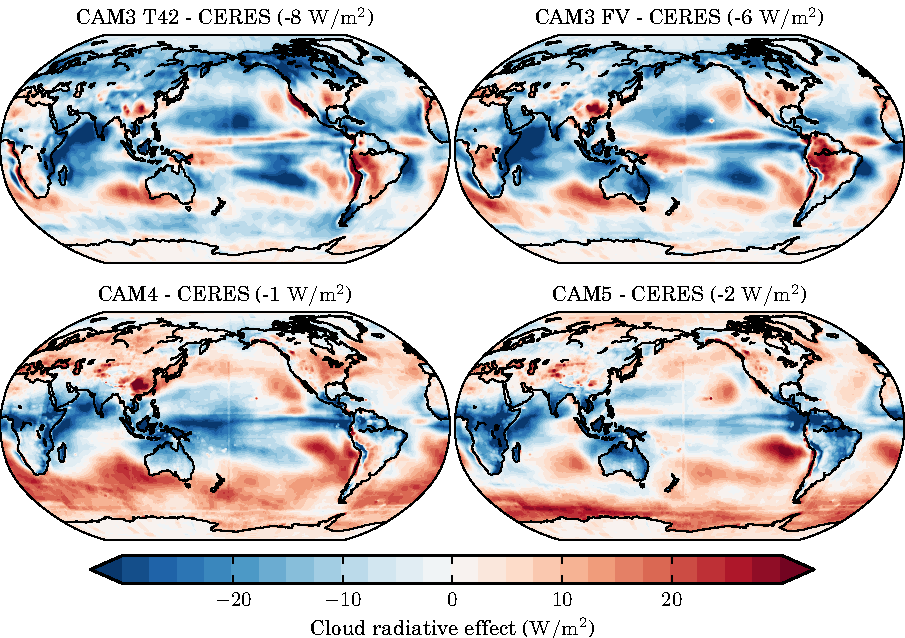
\includegraphics{../graphics/swcrebiases_camamip_map.pdf}
    \caption[Biases in shortwave cloud radiative effect in CAM3, CAM4, and CAM5 AMIP simulations compared with observations from CERES-EBAF.]{Biases in shortwave cloud radiative effect in CAM3, CAM4, and CAM5 AMIP simulations compared with observations from CERES-EBAF. Values in the titles of the individual plots indicate the area-weighted global mean bias between the model and observations.}
    \label{swcrebiases_camamip_map}
\end{figure}

\begin{figure}
    \centering
    \includegraphics{../graphics/lwcrebiases_camamip_map.pdf}
    \caption[Biases in longwave cloud radiative effect in CAM4 and CAM5 AMIP simulations compared with observations from CERES-EBAF.]{Biases in longwave cloud radiative effect in CAM3, CAM4, and CAM5 AMIP simulations compared with observations from CERES-EBAF. Values in the titles of the individual plots indicate the area-weighted global mean bias between the model and observations.}
    \label{lwcrebiases_camamip_map}
\end{figure}

The agreement in the shortwave and longwave cloud radiative effect between all model simulations and observations is summarized in Figure \ref{cre_camamip_taylor}. This figure shows that the correlation improves in each successive version of CAM, although the spatial-temporal variability of the shortwave cloud radiative effect most closely matches the CERES-EBAF observations in the CAM4 simulation. The mean biases compared to the CERES-EBAF dataset are also lower in the CAM4 simulation than for the other model simulation shown here. All model simulations overestimate the magnitude of the shortwave cloud radiative effect (indicated by negative mean biases in each comparison in Figure \ref{swcrebiases_camamip_map}). Figure \ref{lwcrebiases_camamip_map} shows that the CAM3 simulations show an overestimation of the magnitude of the longwave cloud radiative effect, while the CAM4 and CAM5 simulations show an overall underestimation.

The correlation between the ERBE and CERES-EBAF datasets is much higher than that between any of the models and the CERES-EBAF dataset, giving confidence in conclusions drawn regarding the spatial-temporal correlation between model simulations and observations. The ratio of the variances and the relative ``biases'' in these fields between the ERBE dataset and the CERES-EBAF dataset are comparable with those seen in the comparisons between the model simulations and the CERES-EBAF dataset, giving less confidence in the robustness of conclusions drawn regarding these statistical quantities (though it should be noted that the ERBE dataset is only four years in length). The main conclusion from Figure \ref{cre_camamip_taylor}, is that the shortwave and longwave cloud radiative effect is better correlated with observations in space and time in CAM5 than in the two previous versions of CAM.
\begin{figure}
    \centering
    \includegraphics{../graphics/cre_camamip_taylor.pdf}
    \caption[Taylor diagrams comparing shortwave and longwave cloud radiative effect from CAM3, CAM4, and CAM5 AMIP simulations with observations from CERES-EBAF.]{Taylor diagrams comparing shortwave and longwave cloud radiative effect from CAM3, CAM4, and CAM5 AMIP simulations with observations from CERES-EBAF. Shortwave and longwave cloud radiative effect from the Earth Radiative Budget Experiment (ERBE) \citep{harrison_et_al_1990} are compared against the CERES-EBAF dataset as well.}
    \label{cre_camamip_taylor}
\end{figure}

Total, low, middle, and high-topped cloud amounts from ISCCP, MISR, and MODIS and their corresponding simulator diagnostics from CAM3, CAM4, and CAM5 AMIP simulations are shown in Figure \ref{cldtypes_camamip_bar}. As seen in the CAM3 and AM2 evaluation, total and low-topped cloud is underestimated in all models simulations. This is consistent with previous studies identifying underestimation of cloudiness in models \citep{zhang_et_al_2005}. Mid-topped cloud is underestimated in all model simulations except for in CAM5, which shows greatly reduced biases in ISCCP and MISR-simulated mid-topped cloud and a positive bias in MODIS-simulated mid-topped cloud. This result has been documented in \cite{kay_et_al_2011}, and shows that the long-standing negative bias in model-simulated, mid-topped cloud amount identified in \cite{zhang_et_al_2005} is reduced in CAM5, although differences in the sign of the bias when the MODIS comparison is added to the analysis are suggestive of uncertainty in these comparisons. High-topped cloud in CAM5 is shown here to be generally underestimated compared with the observations, while high-topped cloud is generally overestimated in the CAM3 simulations. Biases in ISCCP and MISR-simulated high-topped cloud are also negative in CAM4, although MODIS-simulated high-topped cloud is overestimated. 
\begin{figure}
    \centering
    \includegraphics{../graphics/cldtypes_camamip_bar.pdf}
    \caption[Total, low-topped, mid-topped, and high-topped cloud amount from ISCCP, MISR, and MODIS and corresponding simulator diagnostics from CAM3, CAM4, and CAM5 AMIP simulations.]{Total, low-topped, mid-topped, and high-topped cloud amount from ISCCP, MISR, and MODIS and corresponding simulator diagnostics from CAM3, CAM4, and CAM5 AMIP simulations. MODIS cloud amounts are taken before clear-sky restoral.}
    \label{cldtypes_camamip_bar}
\end{figure}

Statistics for ISCCP, MISR, and MODIS-simulated total, low, mid, and high-topped clouds are compared with ISCCP, MISR, and MODIS observations in Figure \ref{cldtypes_camamip_taylor}. The different cloud types show at best moderate spatial-temporal correlation with observations, relative to the spatial-temporal correlation between the observations of total cloud amount shown in Figure \ref{cldtot_obs_taylor}. Nonetheless, CAM5 shows systematically better correlation with observations in almost every cloud type. Variance ratios between CAM5 and observed cloud types are also improved, indicating a spatial-temporal variability in CAM5 clouds that more closely matches the spatial-temporal variability in observations.
\begin{figure}
    \centering
    \includegraphics{../graphics/cldtypes_camamip_taylor.pdf}
    \caption[Taylor diagrams comparing total, low-topped, mid-topped, and high-topped ISCCP, MISR, and MODIS-simulated cloud amounts from CAM3, CAM4, and CAM5 AMIP simulations with the corresponding satellite retrievals.]{Taylor diagrams comparing total, low-topped, mid-topped, and high-topped ISCCP, MISR, and MODIS-simulated cloud amounts from CAM3, CAM4, and CAM5 AMIP simulations with the corresponding satellite retrievals. MODIS cloud amounts are taken before clear-sky restoral.}
    \label{cldtypes_camamip_taylor}
\end{figure}

As shown in the previous chapter, CAM3 and AM2 compensate for the underestimation of total and low-topped cloud with a high bias in cloud optical thickness. A principle result of the \cite{kay_et_al_2011} study is the reduction of the cloud optical thickness bias in the CAM5 simulation relative to the CAM4 simulation and to other models documented in the literature \citep[e.g.,][]{zhang_et_al_2005}. This result is demonstrated in Figure \ref{tau_camamip}. Both CAM3 and CAM4 simulations underestimate the amount of optically thin and optically intermediate cloud while overestimating the amount of optically thick cloud. This comparison also shows a large difference between the CAM3 and CAM4 simulations. Both have a similar bias in the distribution of cloudiness toward higher optical thickness, but the CAM4 simulation has a much lower amount of cloud with optical thickness $23.0 < \tau < 60.0$. The increased negative bias in cloud amount in CAM4 relative to CAM3 is primarily due to a reduction in this optically thick cloud.

\begin{figure}
    \centering
    \includegraphics{../graphics/tau_camamip.pdf}
    \caption{Global annual mean histograms of cloudiness with cloud optical thickness from ISCCP, MISR, and MODIS and the corresponding simulator diagnostics from CAM3, CAM4, and CAM5 AMIP simulations.}
    \label{tau_camamip}
\end{figure}
\begin{figure}
    \centering
    \includegraphics{../graphics/cth_camamip.pdf}
    \caption{Global annual mean histograms of cloudiness with cloud top height from MISR and the MISR simulator diagnostic from CAM3, CAM4, and CAM5 AMIP simulations.}
    \label{cth_camamip}
\end{figure}


Figure \ref{cth_camamip} shows that the distribution of MISR-simulated cloudiness with cloud top height in the CAM5 simulation more closely matches observations than previous versions of the model. A surprising result illustrated by Figure \ref{cth_camamip} is the difference in the distribution of MISR-simulated cloudiness with cloud top height in the CAM4 simulation relative to the two CAM3 simulations, despite the fact that these models use similar subgrid-scale parameterizations. The distributions from the two CAM3 simulations show a large frequency of cloud with cloud tops below $0.5$ km and a sharp decline between $0.5$ km and $1.0$ km, while the distribution from the CAM4 simulation shows an increase in frequency over this entire range. Due to the finite vertical resolution in the models, the histogram binning can exacerbate the impact of differences in the vertical structure on these comparisons. When relatively few model levels coincide with a vertical histogram bin, small changes in the vertical structure of clouds between models could shift a large population of cloud to adjacent histogram bins. Figure \ref{cl_camamip} shows the distribution of the model-diagnosed cloud amount with vertical level (\emph{not} instrument-simulated). This figure demonstrates that CAM3 and CAM4 do in fact simulate different distributions of cloud as seen by the model. It is also important to keep in mind that the diagnosis of MISR-simulated cloudiness depends not only on the model cloud fraction, but on the optical thickness and emissivity on model levels as well, and differences in these quantities may also contribute to differences in the MISR-simulated distributions from CAM3 and CAM4. Nonetheless, Figures \ref{cth_camamip} and \ref{cl_camamip} show that the vertical structure of clouds differs in CAM3 and CAM4. Differences in the distributions of MISR-simulated cloudiness with cloud top height from the CAM3 T42 and CAM3 FV simulations are much smaller than the differences between the distributions from either of the CAM3 simulations and the CAM4 simulation, despite using entirely different dynamical cores. This shows that something beyond a difference in dynamics is responsible for the differences in the distribution of cloudiness with cloud top height between the CAM3 and CAM4 simulations.

\begin{figure}
    \centering
    \includegraphics{../graphics/cl_camamip.pdf}
    \caption{Model-diagnosed cloud fraction by model level from CAM3 and CAM4 AMIP simulations.}
    \label{cl_camamip}
\end{figure}

\subsection{Cloudiness in the tropics and subtropics}
Following the approach of the previous chapter, Figure \ref{cldcth_camamip_gpci} shows the distribution of cloudiness with cloud top height along the GPCI Pacific transect \citep{teixeira_et_al_2011}. The far right side of each plot corresponds to the region just off the coast of California. This region is characterized by large-scale subsidence and persistent stratocumulus. Both CAM4 and CAM5 simulations seem to underestimate cloud in the California stratocumulus region (Table \ref{regions}), as evidenced by Figure \ref{jointHist_camamip_CaliforniaStrat_JJA}. Figure \ref{cldcth_camamip_gpci} shows that at least in the CAM5 simulation, a large part of this is likely due to the stratocumulus being concentrated too close to the coast and breaking up into shallow cumulus too quickly. Despite this, the CAM5 simulation does show a larger cloud amount in this region in closer agreement with the observations than the CAM4 simulation. The increase in cloud amount comes primarily from an increase in low-topped optically intermediate cloud, as shown by Figure \ref{jointHist_camamip_CaliforniaStrat_JJA}. This, combined with a decrease relative to the CAM4 simulation of low-topped optically thick cloud brings the distribution of cloudiness with cloud optical thickness in this region in CAM5 closer to observations, as noted by \cite{kay_et_al_2011}, but optically thin cloud is still underestimated in this region.

\begin{figure}
    \centering
    \includegraphics{../graphics/cldcth_camamip_gpci.pdf}
    \caption[Histograms of summertime cloudiness with cloud top height along the GPCI Pacific transect from MISR and the MISR simulator diagnostic from CAM4 and CAM5 AMIP simulations.]{Histograms of summertime (June, July, August) cloudiness with cloud top height along the GPCI Pacific transect from MISR and the MISR simulator diagnostic from CAM4 and CAM5 AMIP simulations.}
    \label{cldcth_camamip_gpci}
\end{figure}

Stratocumulus in the CAM5 simulation seems to transition too early into the cumulus regime, while the CAM4 simulation shows a uniform vertical and geographic distribution of cloudiness from the stratocumulus region to about $20~^\circ\text{N}$, where a sharp transition occurs. This transition in the CAM4 simulation is similar to that seen in the CAM3 simulation. None of the simulations capture the rising of cloud tops in the transition from stratocumulus to trade cumulus.

\begin{figure}
    \centering
    \includegraphics{../graphics/hist2d_camamip_california.pdf}
    \caption[California stratocumulus joint histogram of summertime cloudiness with cloud optical thickness and cloud top height from MISR, ISCCP, and MODIS and the corresponding simulator diagnostics from CAM4 and CAM5 AMIP simulations.]{California stratocumulus (Table \ref{regions}) joint histogram of summertime (June, July, August) cloudiness with cloud optical thickness and cloud top height (or pressure) from MISR, ISCCP, and MODIS and the corresponding simulator diagnostics from CAM4 and CAM5 AMIP simulations.}
    \label{jointHist_camamip_CaliforniaStrat_JJA}
\end{figure}

The far left side of Figure \ref{cldcth_camamip_gpci} corresponds to the deep convective region in the central Pacific in the ITCZ. Both model versions seem to overestimate the amount of high-topped cloud in this region. This bias in high-topped cloud amount results in a large positive bias in the longwave cloud radiative effect in this region in CAM3, CAM4 and, to a lesser extent, in CAM5. This bias does not exist in in the tropical western Pacific region (Figure \ref{jointHist_camamip_TropicalWPacific_JJA}) in either model, although the distribution of cloudiness is biased toward higher optical thickness throughout the vertical in both CAM4 and CAM5 model simulations, similar to that demonstrated in the previous chapter for the CAM3 and AM2 simulations. This bias is reduced in the CAM5 simulation, which brings the distribution closer to observations.

\begin{figure}
    \centering
    \includegraphics{../graphics/hist2d_camamip_twp.pdf}
    \caption[Tropical western Pacific joint histogram of summertime cloudiness with cloud optical thickness and cloud top height from MISR, ISCCP, and MODIS and the corresponding simulator diagnostics from CAM4 and CAM5 AMIP simulations.]{California stratocumulus (Table \ref{regions}) joint histogram of summertime (June, July, August) cloudiness with cloud optical thickness and cloud top height (or pressure) from MISR, ISCCP, and MODIS and the corresponding simulator diagnostics from CAM4 and CAM5 AMIP simulations.}
    \label{jointHist_camamip_TropicalWPacific_JJA}
\end{figure}

Both CAM4 and CAM5 do simulate the cloud layer associated with the tropical freezing level \citep{johnson_et_al_1999} seen in the MISR observations, although both simulations overestimate the amount of this cloud. This cloud layer is not seen in the CAM3 simulation, so this represents an improvement from CAM3.

\section{Discussion}
Diagnostics using satellite instrument simulators are useful tools in evaluating the representation of clouds in climate models and assessing changes in cloud properties associated with the introduction of new model formulations. The results shown here provide a compliment to those presented in \cite{kay_et_al_2011} by focusing on output from the passive sensor instrument simulators and extending the analysis to assess changes since CAM3.

The use of satellite instrument simulators in this study allows for evaluation of model performance using multiple independent observational datasets quantifying clouds and their radiative properties. Compensating biases in the cloud properties are exposed that may permit reasonable estimates of top of atmosphere energy fluxes with cloud property statistics that differ from reality. In particular, the models studied here have a tendency to compensate for an underestimation of cloud amount with an overestimation of cloud optical thickness. The overestimation of optically thick and the underestimation of optically thin clouds is a common model bias \citep{zhang_et_al_2005}. Changes made in the formulation of CAM5 have reduced the global annual mean bias in simulations with this model.

Total cloudiness is chronically underestimated in all three CAM versions, largely due to underestimation of low and mid-topped cloud. This is especially true for CAM3 and CAM4. The underestimation of mid-topped and, to a lesser extent, low-topped cloud is another common model bias documented in \cite{zhang_et_al_2005}. These biases are greatly reduced in CAM5. \cite{kay_et_al_2011} increase the robustness of this result by adding comparisons with CALIPSO observations.

Despite the improvement in the CAM5 representation of clouds by nearly every measure documented here, large biases remain. Regional biases remain in the cloud properties themselves and in their impact on top of atmosphere radiative fluxes as quantified by the shortwave and longwave cloud radiative effect. Spatial and temporal correlations of these properties between model and observations remain well below correlations between the different observational sets.

Simulation of boundary layer clouds in regions of large-scale subsidence remains troublesome in CAM4 and CAM5. Studies such as that of \cite{bony_and_dufresne_2005} point to the importance of these cloud types to tropical feedbacks. This suggests that efforts to improve the representation of these cloud types in CAM5 will be important.

Despite sharing many physical parameterizations there are substantial differences in the simulation of clouds in CAM3 and CAM4. Experiments substituting the dynamical core in CAM3 suggest that the causes of the changes are rooted elsewhere. It is important to track down the source of these discrepancies as situations such as this provide an opportunity to gain insight into the effect of different changes in the model formulation on the simulation of clouds in climate models. These changes will be invested further in future work.

\chapter{CAM3 and AM2 cloud response to warming}
\label{cmip3hot}
\section{Introduction}
The simulated climate response to increases in carbon dioxide is known to differ among different climate models. For the past two decades, cloud feedback processes have been recognized as being among the largest sources of inter-model spread in equilibrium climate sensitivity and in uncertainty in future projections of the earth climate system made by climate models \citep{cess_et_al_1990,cess_et_al_1996,colman_2003,soden_and_held_2006,webb_et_al_2006,ar4_ch8}. \cite{stephens_2005} argues that much of the uncertainty in cloud feedbacks in climate models stems from the difficulty in representing cloud processes in model simulations, due to the discrepancy in resolution between that which is practical for global-scale climate models and that which is important for cloud-related processes. The result is that these processes must be parameterized to approximate their effects at the relatively coarse resolution of climate models. \cite{randall_et_al_2003} describe this so-called parameterization problem as an attempt to represent the small-scale effects, such as clouds, in terms of the large-scale system. This is a difficult process as the connection between effects at the two scales is not constrained by a single physical theory, and different modelers may take different approaches to the problem. The high level of empiricism and differences in approach to this problem leads to high levels of uncertainty in the representation of clouds in climate models and especially in the simulated responses of clouds to climate change. Numerous studies have demonstrated that the sensitivity of climate models depends on the representation of clouds \citep[e.g.,][]{mitchell_et_al_1987,senior_and_mitchell_1993,le_treut_et_al_1994,fowler_and_randall_1994,ma_et_al_1994,liang_and_wang_1997,yao_and_del_genio_2002,zhang_2004,stainforth_et_al_2005,yokohata_et_al_2005}, and \cite{stephens_2005} emphasizes the critical importance of progress on the cloud parameterization problem to the progress of the cloud feedback problem. 

Evaluations of model simulated clouds for present day climate simulations are an important first step toward assessing the representation of clouds in climate models. Evaluating the response of climate model simulations to climate change scenarios is nontrivial, as observational data is not available for comparison. This leaves open the question of how clouds can be expected to respond to a changing climate, and numerous hypotheses have been suggested.

The tropics are characterized by large over-turning circulations, giving rise to regions of deep convection and associated anvil-forming clouds, and regions of subsidence and associated boundary layer clouds. How such convective anvil clouds should respond to climate change has been the subject of a number of studies and hypotheses. The ``Fixed-Anvil Temperature'' (FAT) hypothesis of \cite{hartmann_and_larson_2002} suggests that the temperature of the tops of these anvil clouds is essentially independent of the surface temperature, and that their temperature can be expected to remain nearly constant even as surface temperatures rise. The heights of the anvil cloud tops rise in order to stay at the same temperature. This mechanism implies a positive feedback, as the temperature difference between high-topped clouds and the surface increases in a warming climate, leading to an enhanced longwave heating effect. Evidence supporting the fixed-anvil temperature hypothesis has been demonstrated in cloud resolving models \citep{kuang_and_hartmann_2007}, and more recently in climate models \citep{zelinka_and_hartmann_2010}.

There is considerable disagreement on the likely response of the amount of anvil cloud fraction to climate change \citep{ar4_ch8}. The so-called ``iris'' hypothesis \citep{lindzen_et_al_2001} suggests that anvil cloud amount would decrease in response to increasing sea surface temperatures and cause a negative feedback, but this hypothesis has met much criticism \citep{chambers_et_al_2002,del_genio_and_kovari_2002,fu_et_al_2002,harrison_2002,hartmann_and_michelsen_2002,lin_et_al_2002,lin_et_al_2004}.

The response of boundary layer clouds to climate change is not yet well understood \citep{ar4_ch8}. An observed correlation between low-level cloud amount and lower tropospheric stability \citep{klein_and_hartmann_1993} has inspired studies suggesting that low-level cloud amount should increase with increasing sea surface temperature, providing a negative feedback by increasing the shortwave cooling effect of clouds \citep{miller_1997,zhang_2004}, although these results are uncertain. Observational studies have suggested that optical thickness decreases in regions covered by low-level clouds with increasing temperatures, decreasing the shortwave cooling effect of clouds \citep{tselioudis_and_rossow_1994,greenwald_et_al_1995,bony_et_al_1997,del_genio_and_wolf_2000,bony_and_dufresne_2005}. In a warming climate, this would provide a positive feedback, although \cite{ar4_ch8} note again that understanding of this is limited.

\section{Model and experiment set-up}
A simple experiment design to analyze feedbacks was proposed by \cite{cess_and_potter_1988}. It uses a uniform sea surface temperature perturbation as a surrogate for climate change. In this design, the climate change is essentially prescribed, and the response of the system to the prescribed change can be studied. This concept has been used in a number of studies to study feedbacks \cite[e.g.,][]{cess_et_al_1990,cess_et_al_1996}, but others have pointed to differences in feedbacks calculated using the methods of \cite{cess_and_potter_1988} and traditional full feedback calculations using coupled models \citep{senior_and_mitchell_1993,soden_et_al_2004,ringer_et_al_2006}. More recently, \cite{gettelman_et_al_2011} looked at feedbacks in two recent versions of the NCAR CAM using a similar experiment design, but replacing the uniform sea surface temperature perturbation with a spatially varying perturbation determined from a slab ocean model climate change simulation.

Despite the limitations of the method proposed by \cite{cess_and_potter_1988} for diagnosing feedbacks, the concept of using a sea surface temperature perturbation as a surrogate for climate change has proven to be quite useful. This concept is used here to assess the changes in clouds in response to a prescribed climate change in the two models evaluated in Chapter \ref{cmip3amip}. Each model is forced with the same observed, monthly-evolving sea surface temperatures used in the AMIP simulations, but with a uniform $+4~\text{K}$ temperature perturbation applied. A $+4~\text{K}$ perturbation was used rather than the typical $\pm 2~\text{K}$ perturbation used in previous feedback studies in order to increase the signal using only a single simulation. These ``HOT4K'' simulations were run for the ten-year period from 1990-1999, with a one-year spin-up started in 1989 not included in the reported climatologies.

The response of the clouds in the perturbed sea surface temperature simulations are assessed using satellite instrument simulators. The benefit of using satellite instrument simulators in this case is not to facilitate comparisons between model and observations, as observations are not available for the perturbed climate. Rather, the simulator approach allows comparisons of radiatively important cloud statistics between the control and perturbed model climates, as well as providing a common framework in which to compare the responses of the two models. In addition, this approach gives at least an estimate of how the real-world clouds might be expected to respond as seen by the available instruments in a similarly perturbed climate, and gives some insight into the ability of these instruments to detect changes in the clouds brought about by climate change.

\section{Results}
The NCAR CAM3 and GFDL AM2 are chosen for this study in large part because of their known differing responses to climate change (e.g. \cite{stephens_2005}, Figure 1, although this is an earlier version of the CAM than used here). This is immediately apparent in Figures \ref{swcrechanges_cmip3hot4k_map} and \ref{lwcrechanges_cmip3hot4k_map}, which show the changes in the shortwave and longwave cloud radiative effect between the AMIP and HOT4K simulations. The changes in both the regional and globally averaged shortwave and longwave cloud radiative effect terms are quite different between the two models. The CAM3 simulation shows an increase in the magnitude of both the global annual mean shortwave and longwave cloud radiative effect, while the AM2 simulation shows no appreciable change in the global annual mean. 

The differences in the regional responses of the two models are more dramatic. The CAM3 simulation shows an enhancement of both the shortwave and longwave cloud radiative effect through much of the tropical Pacific Ocean and into the southern hemisphere trade cumulus. In contrast, the AM2 simulation shows a weakening of the magnitude of the shortwave cloud radiative effect throughout the subtropical stratocumulus and trade cumulus regions, with an increase in magnitude of the shortwave cloud radiative effect along the ITCZ and in the tropical warm pool.

\begin{figure}
    \centering
    \includegraphics{../graphics/swcrechanges_cmip3hot4k_map.pdf}
    \caption{Changes in shortwave cloud radiative effect between AMIP and HOT4K simulations from CAM3 and AM2.}
    \label{swcrechanges_cmip3hot4k_map}
\end{figure}

\begin{figure}
    \centering
    \includegraphics{../graphics/lwcrechanges_cmip3hot4k_map.pdf}
    \caption{Changes in longwave cloud radiative effect between AMIP and HOT4K simulations from CAM3 and AM2.}
    \label{lwcrechanges_cmip3hot4k_map}
\end{figure}


The decrease in magnitude of the shortwave cloud radiative effect in the subtropical marine stratocumulus regions in the AM2 simulation is explained by Figure \ref{hist2d_cmip3hot4k_california}, which shows that low-topped cloud in the California stratocumulus region decreases in the perturbed climate relative to the AMIP simulation. The largest change in cloudiness occurs for low-topped optically intermediate cloud, and in the bins with the highest frequency of occurrence in the AMIP simulation (Figure \ref{hist2d_cmip3amip_california}). In contrast the CAM3 perturbed sea surface temperature simulation shows much less change in low-topped cloud in this region summed across all optical thickness bins, but the distribution with optical thickness has changed, as shown by the increase in low-topped optically thick cloud and the decrease in low-topped optically intermediate cloud. This loosely follows the pattern of the bias in the simulation of the present day climate, which shows a bias toward cloud with higher optical thickness than observed by any of the three instruments considered.

\begin{figure}
    \centering
    \includegraphics{../graphics/hist2d_cmip3hot4k_california.pdf}
    \caption[California stratocumulus changes in summertime cloudiness with cloud top height and optical thickness between AMIP and HOT4K simulations from CAM3 and AM2.]{California stratocumulus (Table \ref{regions}) changes in summertime (June, July, August) cloudiness with cloud top height and optical thickness between AMIP and HOT4K simulations from CAM3 and AM2.}
    \label{hist2d_cmip3hot4k_california}
\end{figure}

The decrease in the magnitude of the shortwave cloud radiative effect in the Hawaiian trade cumulus in the AM2 simulation is consistent with an overall decrease in cloud amount in this region, especially in high-topped optically thin and low-topped optically intermediate cloud types (Figure \ref{hist2d_cmip3hot4k_hawaiian}). As in the California stratocumulus, the cloud types that change the most are those that have the highest frequency of occurrence in the AMIP simulation, and also represent the cloud types with large biases relative to the observations in the AMIP simulation. The response of the CAM3 simulation again differs from the response of the AM2 simulation. High-topped optically thin cloud decreases similarly, but this is largely compensated for in the CAM3 simulation by an increase in high-topped optically thick cloud, with the net result being much less change in high-topped cloud than seen in the AM2 simulation. The response of the low-topped cloud is quite different in the CAM3 simulation, with a large increase in low-topped cloud mainly due to an increase in low-topped optically thick cloud. Again, the cloud types with the largest changes in the perturbed sea surface temperature simulation seem to be those that occur with large frequency in the AMIP simulations.

\begin{figure}
    \centering
    \includegraphics{../graphics/hist2d_cmip3hot4k_hawaiian.pdf}
    \caption[Hawaiian trade cumulus changes in summertime cloudiness with cloud top height and optical thickness between AMIP and HOT4K simulations from CAM3 and AM2.]{Hawaiian trade cumulus (Table \ref{regions}) changes in summertime (June, July, August) cloudiness with cloud top height and optical thickness between AMIP and HOT4K simulations from CAM3 and AM2.}
    \label{hist2d_cmip3hot4k_hawaiian}
\end{figure}

In the deep tropics, both CAM3 and AM2 simulations show increases in the magnitude of both the shortwave and longwave cloud radiative effect, although the increase is much more substantial and widespread in the CAM3 simulation (Figures \ref{swcrechanges_cmip3hot4k_map} and \ref{lwcrechanges_cmip3hot4k_map}). These changes are due to large changes in the high-topped clouds in this region, as shown for the tropical western Pacific in Figure \ref{hist2d_cmip3hot4k_twp}. The increase in the shortwave cloud radiative effect in both CAM3 and AM2 simulations in this region is likely due to the large increases in high-topped optically thick cloud. High-topped optically thick cloud increases more in the CAM3 simulation, causing the larger increase in the shortwave cloud radiative effect seen in Figure \ref{swcrechanges_cmip3hot4k_map}. The increase in high-topped optically thick cloud is partially compensated for in both model simulations by a decrease in high-topped optically thin cloud. In the CAM3 simulation, the increase in high-topped optically thick cloud is greater in magnitude than the decrease in high-topped optically thin cloud, easily explaining the large increase in the magnitude of the longwave cloud radiative effect in this region. The increase in high-topped optically thick and decrease in high-topped optically thin clouds are much closer in magnitude in the AM2 simulation and, in fact, the MODIS simulated cloud actually shows an overall decrease in high-topped cloud. The increase in longwave cloud radiative effect is instead accounted for by an increase in cloud top heights of high-topped cloud in this region. This is clearly demonstrated in the MISR and MODIS-simulated joint histograms of change of cloudiness with cloud top height and optical thickness (upper and lower-right panels of Figure \ref{hist2d_cmip3hot4k_twp}), which show an increase in frequency of high-topped clouds in bins directly above bins that show a corresponding decrease in frequency. Evidence for an upward shift in cloud top heights is seen in the CAM3 perturbed sea surface temperature simulation as well. This rise in cloud top heights is consistent with that predicted by the fixed-anvil temperature hypothesis \citep{hartmann_and_larson_2002,zelinka_and_hartmann_2010}.

\begin{figure}
    \centering
    \includegraphics{../graphics/hist2d_cmip3hot4k_twp.pdf}
    \caption[Tropical western Pacific changes in northern hemisphere summertime cloudiness with cloud top height and optical thickness between AMIP and HOT4K simulations from CAM3 and AM2.]{Tropical western Pacific (Table \ref{regions}) changes in northern hemisphere summertime (June, July, August) cloudiness with cloud top height and optical thickness between AMIP and HOT4K simulations from CAM3 and AM2.}
    \label{hist2d_cmip3hot4k_twp}
\end{figure}

\section{Discussion}
The two models considered here have very different cloud responses in regions dominated by boundary layer clouds in the subtropics. Large biases in these cloud types were demonstrated earlier in simulations of present day climate from both models, and their differing responses to increasing sea surface temperatures demonstrated here underscores the concern raised earlier as to the credibility of cloud feedbacks represented by these models. The very differing responses of clouds in these regions is consistent with the implication of \cite{bony_and_dufresne_2005} that the response of these clouds to surface warming are the main source of uncertainty in tropical cloud feedbacks.

Cloud top heights in the deep tropics increase in response to increased sea surface temperatures in both models. This result is consistent with the fixed-anvil temperature hypothesis \citep{hartmann_and_larson_2002}, and explains the increase in the magnitude of longwave cloud radiative effect in the deep tropics in both models. \cite{zelinka_and_hartmann_2010} showed that the cloud top heights of high-topped clouds in the tropics similarly increase in IPCC SRES A2 scenario simulations. The CAM3 simulation also shows a large increase in high-topped optically thick cloud in this region, which is likely to be of greater impact on the longwave cloud radiative effect than the increase of cloud top heights in this region.

Using satellite instrument simulators in the study of the response of clouds to increasing sea surface temperatures provides a common framework for the intercomparison of models, but perhaps more importantly allows for changes in the simulation of the perturbed climate to be assessed in relation to identified biases in the simulation of present day climate. An important result demonstrated here using this technique is that some of the largest changes in the clouds in response to an increase in sea surface temperatures seem to occur in cloud types with have a high frequency of occurrence and large biases in present day climate simulations. It is unclear from this study whether this represents a model tendency for responses to climate change to track the inherent model biases, or is simply due to the fact that these cloud types have the highest potential to change due to their high relative occurrence. This question will be the focus of further studies.

\chapter{Summary and Future Work}
The representation of clouds in climate models is of critical importance to the simulation of climate. The use of satellite instrument simulators enables the type of robust and quantitative evaluation of the simulation of clouds in climate models against observations performed in this study.

Climate models are broadly constrained to achieve net energy balance at the top of the atmosphere. Although this is a necessary requirement to prevent simulated climates that are unstable and unphysical, it fails to constrain the individual effects that combine to produce the net balance, leaving room for potentially compensating errors in other quantities. In particular, although the net radiation balance is constrained, no constraints are placed on the total cloud amount, the vertical distribution of cloudiness, or on the cloud properties themselves. Quite often the cloud properties are used as tuning parameters and clouds are adjusted to enable the model to match the top of atmosphere energy balance. The presence of compensating biases in the cloud radiative properties in climate models has been suggested by others \citep[e.g.,][]{webb_et_al_2001,kay_et_al_2011} and has been demonstrated in this study for two widely used climate models. Recent studies have also pointed to similar biases in the representation of precipitation \citep{stephens_et_al_2010}.

The impact of compensating biases in mean-state simulation of clouds in climate models on cloud feedbacks have not yet been well documented. Using simple sea surface temperature perturbation experiments (which are typically used to diagnose feedbacks following \cite{cess_and_potter_1988}), the response of clouds to a prescribed surface warming has been assessed in this study using the same framework used to evaluate the simulation of clouds in present day climate against observations. This strategy facilitates connecting changes in climate change simulations with identified biases in simulations of the mean-state climate. The most substantial changes in the clouds in the perturbed climate seem closely related to biases identified in the mean-state climate. This has shown that the utility of the instruments simulators extends beyond evaluation of mean-state climate by providing a framework to assess changes associated with climate change consistent with evaluations of mean-state simulations. This also provides a common framework to evaluate a range of models and make inter-comparisons that is useful not only in evaluating the mean-state simulations of a range of models, but in comparing responses of different models to climate change using consistent diagnostics.

Although the presence of compensating biases has been identified in this study, quantification of the effect of individual biases on the top of atmosphere radiative fluxes has not been attempted. \cite{zelinka_thesis} has developed a set of radiative kernels that describe the sensitivity of the top of atmosphere radiative flux to changes in the different cloud types classified by the ISCCP joint histogram. By applying these kernels to biases identified in the ISCCP clouds types, the impact of these different biases on the top of atmosphere radiative fluxes can be quantified. This would allow an assessment of the radiative importance of different biases identified in the mean-state climate simulations. Similar kernels could be computed for cloud types identified by the MISR joint histogram as well.

Techniques used in this study lend themselves to model inter-comparisons of larger scale. Until now a robust evaluation of cloud properties across models has been difficult due to a lack of simple methods that relate the different information provided by satellite retrievals to model output. The ISCCP simulator has alleviated some of these issues, but the use of multiple observations to evaluate models increases the robustness of conclusions drawn from these sorts of comparisons. Comparisons using MISR observations also enable better evaluation of low-topped clouds, while MODIS observations provide a better estimate of mid and high-topped clouds. MODIS observations and the corresponding MODIS simulator also provide an opportunity to evaluate cloud microphysical properties such as effective particle size \citep{pincus_et_al_2011}, but observational uncertainty in some of these observed fields makes this difficult \citep{kay_et_al_2011}. The incorporation of COSP diagnostics in model simulations performed for the Climate Model Intercomparison Project Phase 5 \citep[CMIP5;][]{taylor_et_al_2011} promises to provide an opportunity to robustly evaluate the simulation of clouds in a wide range of climate models in a consistent manner using multiple observational datasets. This will further understanding of the strengths and weaknesses of climate models in simulating clouds, and hopefully drive future development efforts aimed at improving the representation of clouds in climate models.

\printendnotes

%
% ==========   Bibliography
%
%\nocite{*}   % include everything in the uwthesis.bib file

%%% To use AMS guidelines, you need the ametsoc.bst file.
\bibliographystyle{ametsoc}
\bibliography{thesis}

%
% ==========   Appendices
%
%\appendix
%\raggedbottom\sloppy
%\include{appendixa}

\end{document}
